\chapter{GENEL BİLGİLER \label{sec:genel}}

\section{Giriş}
\label{sec:GenelBilgiler_giris}
Pankreas kanseri, ölüm oranı yüksek ve oldukça hızlı seyreden bir kanser türüdür. Pankreas organı vücudumuzda yer aldığı konum itibari ile saklı organ olarak da adlandırılmaktadır ve bu saklı konumu nedeni ile pankreas tümörleri çoğunlukla karın üzerinden el ile kontrolde fark edilememektedir. Bu sebeple pankreas kanserine yakalanan hastaların çoğu hastalık ileri bir aşamaya gelene kadar hastalığa dair belirti göstermemektedirler. Pankreas kanseri semptomları genellikle tümörün mide, on iki parmak bağırsağı, karaciğer veya safra kesesi gibi diğer yakın organların işlevine müdahale etmeye başlayana kadar ortaya çıkmamaktadır. Bu durum kanserin geç teşhis edilmesine sebebiyet vermektedir. Ayrıca yüksek pankreas kanseri riski taşıyan hastaları taramak için ailesinde pankreas kanseri ve kronik pankreatit öyküsü olanların tespit edilmesi gibi standart bir program bulunmamaktadır. Pankreas kanserlerinin çoğu, pankreas içi epitelyal neoplaziler olarak adlandırılan pankreas kanalları içindeki mikroskobik non-invaziv epitel proliferasyonlarından kaynaklanmaktadır \cite{kamisawa2016pancreatic,mizrahi2020pancreatic,hidalgo2010pancreatic}. 

\captionsetup[figure]{margin={0.2cm,0.3cm}}
\begin{figure}[h!]
	\begin{center}
		\vspace{0.4cm}
		\captionbox{SEER 18, (2011-2017) yılları arasında karşılaşılan kanser hastalarının 5 yıllık sağkalım oranları \cite{pancreasistatisticseer2}.
			\label{fig:seer_stat}}
		{
			\vspace{0.4cm}
			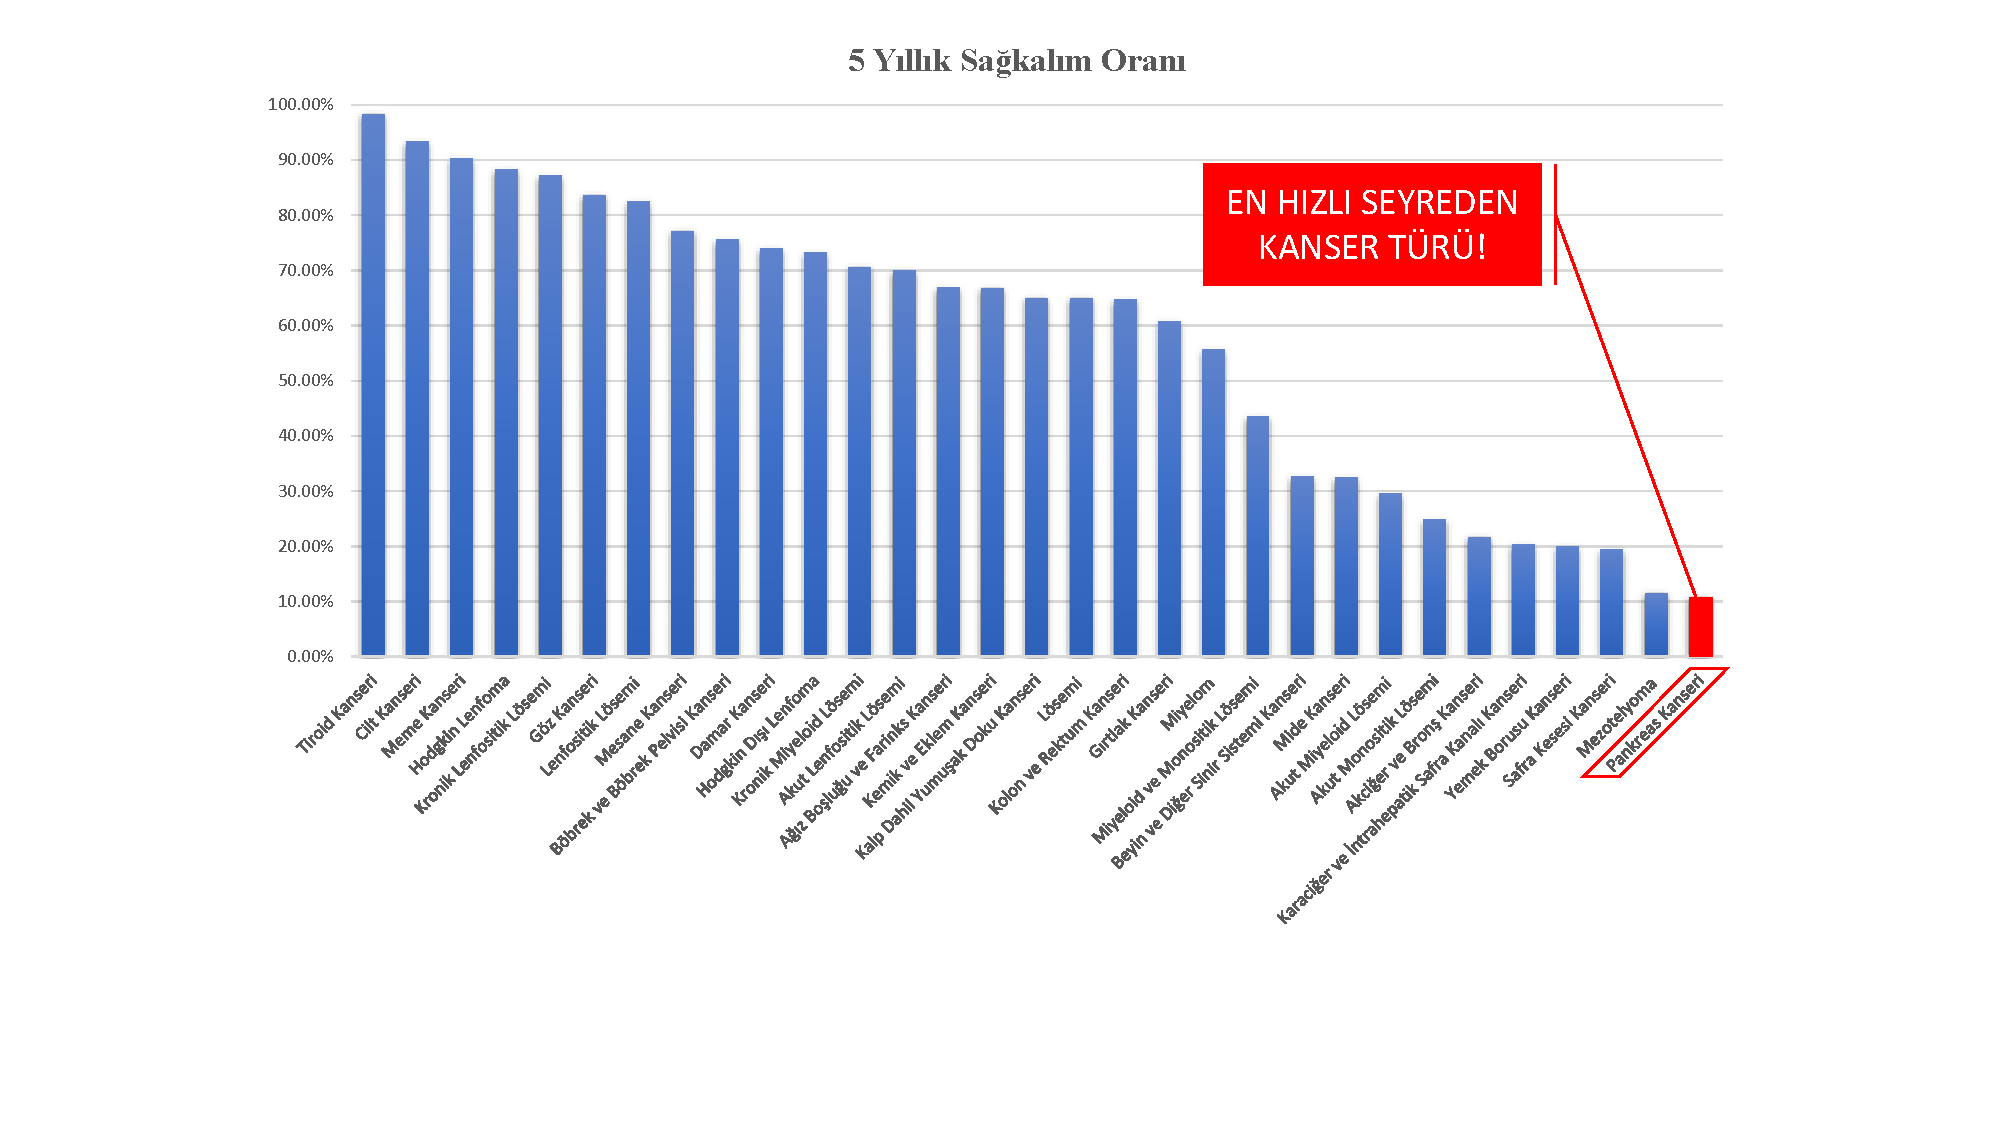
\includegraphics[scale=0.62]{Genel-Bilgiler/Figures/seer_statistic.pdf}
		}
	\end{center}
\end{figure}

Pankreas kanseri sürecinde hastalığa yakalanma ve hastalığa bağlı ölüm arasında geçen süreye bakıldığında, bu sürenin oldukça kısa sürdüğü gözlemlenmektedir. The Surveillance, Epidemiology, and End Results (SEER) Programı Amerika'daki bazı eyaletlerdeki kanser istatistiklerini raporlayan bir kuruluştur \cite{pancreasistatisticseer}. 1973 yılından beri istatistiksel bilgiler bu kuruluş tarafından toplanmakta ve kanser hastalarının istatistiksel verilerinin yorumlanmasına dair en geniş katılımlı ve en güvenilir verileri sağlamaktadır. Şekil \ref{fig:seer_stat}'de verilen SEER 18, (2011-2017) yılları arasında karşılaşılan kanser hastalarının 5 yıllık sağkalım oranlarına bakıldığında en hızlı seyreden kanser türünün pankreas kanseri olduğu görülmektedir. 

Pankreas kanserli hastalarda 5 yıllık sağkalım oranı Amerika Birleşik Devletleri'nde \%10’a kadar düşmektedir. Bu oran diğer kanser türlerine göre oldukça düşüktür. Bu düşük sağkalım oranının en önemli sebebi hastalığın teşhisinin geç konmasıdır. Pankreas kanseri ile mücadele eden hastaların çoğu, hastalık ileri bir aşamaya gelinceye kadar asemptomatiktir.

Pankreas kanseri 5 yıllık sağ kalım oranının bu kadar yüksek olmasının başlıca sebebi erken teşhisinin oldukça zor olmasıdır. Bu sebeple pankreasın konumsal ve şekilsel zorluğu düşünüldüğünde doktorlara yardımcı bir bilgisayar destekli teşhis sisteminin önemi ortaya çıkmaktadır. Pankreas kanserinde ön teşhis genellikle Bilgisayarlı Tomografi (BT), Magnetik Rezonans (MR) gibi volümetrik veri üreten ve doktor tarafından işlenerek çıkarımda bulunulması zahmetli görüntüleme teknikleri ile gerçekleştirilmektedir. Bilgisayar destekli sistemler bu tür verilerin işlenerek doktorların daha kolay çıkarımda bulunabilmelerine imkan tanıyabilmektedir.

\section{Pankreas Organı Konumu ve Görevi}
Pankreas organı salgıladığı enzimler ile sindirim sistemi ve kan şekeri seviyelerinin kritik kontrolünde önemli rol oynayan iki işlevli uzun yassı hormonal bir bezdir \cite{bockman1993anatomy}. Hem iç hem de dış salgı bezi olarak görev yapmaktadır. Bu yüzden karma bez olarak da adlandırılmaktadır. Pankreas organı ortalama olarak 15-25 cm uzunluğuna sahip olup erkeklerde ortalama 75 gr kadınlarda ise ortalama 55 gr ağırlığına sahiptir. Pankreasın düzensiz biçimi önden arkaya doğru yassılaşmakta ve bir çengele benzetilebilmektedir. Pankreas organının anatomik yapısı Şekil \ref{fig:pank_anat}'de verilmektedir. Şekilde görüldüğü gibi pankreas anatomik yapı olarak pankreas adacıkları, safra kanalı, pankreas hormonları ve asiner hücrelerinden oluşmaktadır. İnsülin, glukagon ve somatostanin pankreas hormonlarındandır. Pankreas adacıkları ise alfa, beta ve delta hücrelerinden oluşmaktadır. Yapısal olarak baş, boyun, gövde ve kuyruk olmak üzere temelde 4 ayrı bölgeye ayrılabilmektedir. 

\captionsetup[figure]{margin={0.3cm,0cm}}
\begin{figure}[h!]
	\begin{center}
		\vspace{0.4cm}
		\captionbox{Pankreas organının anatomik yapısı\cite{pancreasimage}
		\label{fig:pank_anat}}
		{
			\vspace{0.4cm}
			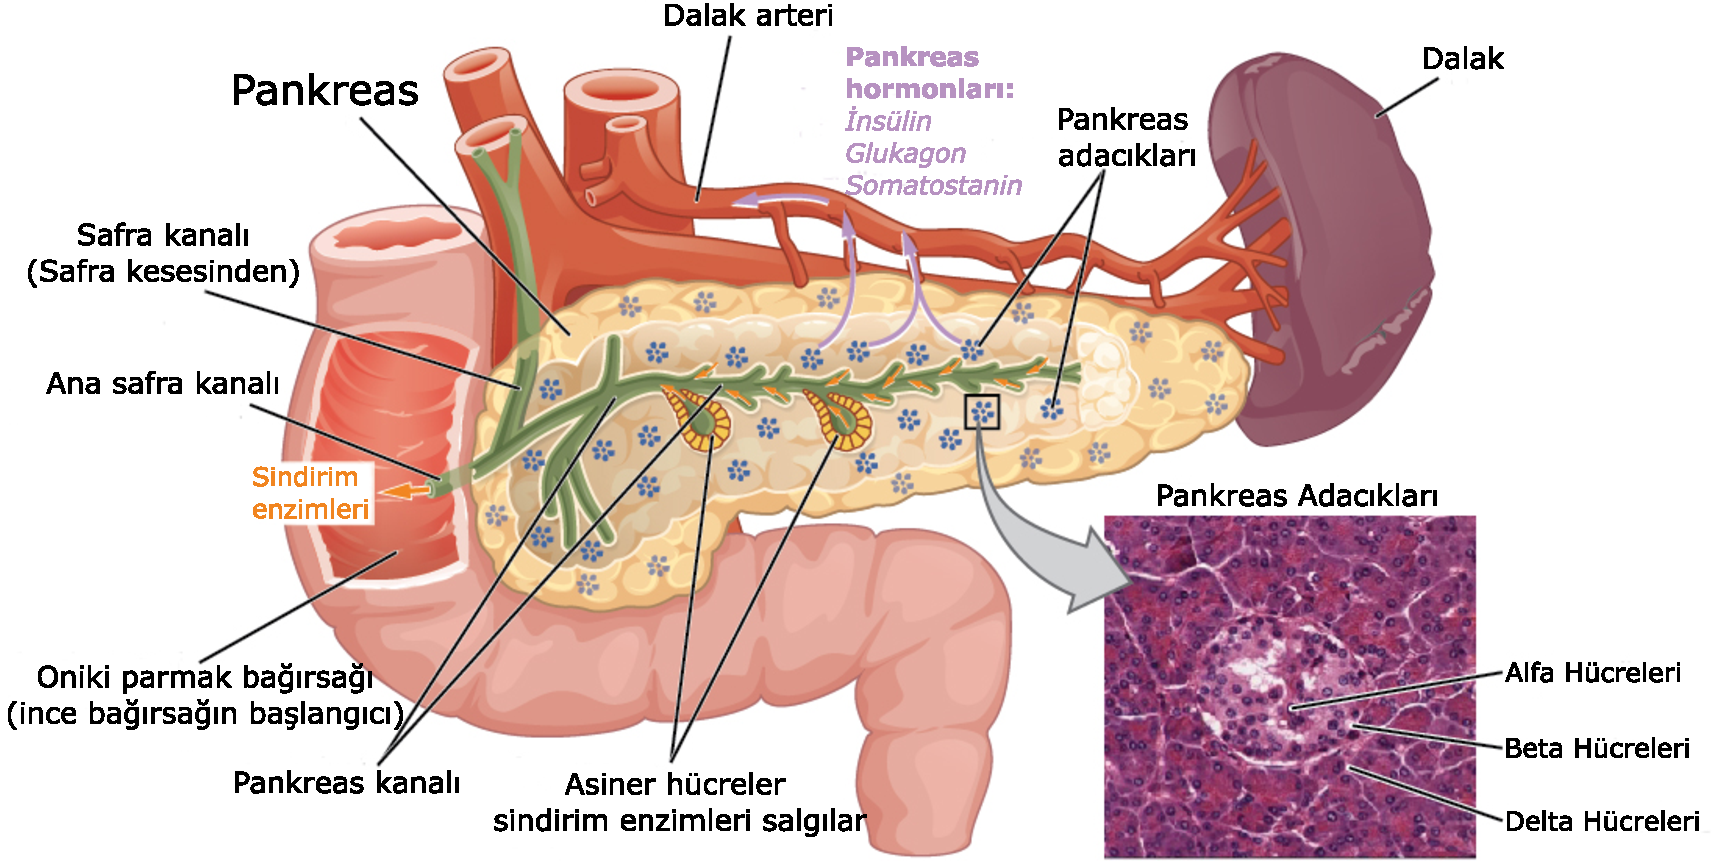
\includegraphics[scale=0.52]{Genel-Bilgiler/Figures/pankreas.pdf}
		}
	\end{center}
\end{figure}

Pankreas organı konumsal olarak bazı önemli ana taşıyıcı damarlara da oldukça yakın pozisyonda bulunmaktadır. Vücudumuzdaki en büyük atardamar olan Aort damarı ve alt ana toplar damar pankreasın baş bölgesinin hemen arkasında kalmaktadır. Ana atar ve toplar damarların geçtiği kodumda yer almasından dolayı yine birçok önemli damar ile birebir ilişki içerisindedir. Bu sebeple pankreas organında ortaya çıkan kitleler aşırı büyüdüğünde önemli damarların daralmasına ve buna bağlı olarak sarılık, damar tıkanıklığı gibi oldukça ölümcül hastalıklara sebebiyet verebilmektedir.

Şekil \ref{fig:pank_konum}’ de görüldüğü gibi pankreas organı konum olarak abdominal (karın, göbek) bölgede yer almaktadır.  Pankreas organı karnın arka bölümünün ortasında olup, sağ kısmı mide ile omurga arasında yer alırken, kuyruk kısmı soldan on iki parmak bağırsağının kıvrımına (ince bağırsağın ilk kısmı) kadar uzanmaktadır \cite{bockman1993anatomy,skandalakis1993surgical}.

\captionsetup[figure]{margin={0.9cm,0cm}}
\begin{figure}[h!]
	\begin{center}
		\vspace{0.4cm}
		\captionbox{Pankreas organının vücuttaki konumu \cite{pancreaslocationimage}
		\label{fig:pank_konum}}
		{
		    \vspace{0.1cm}
			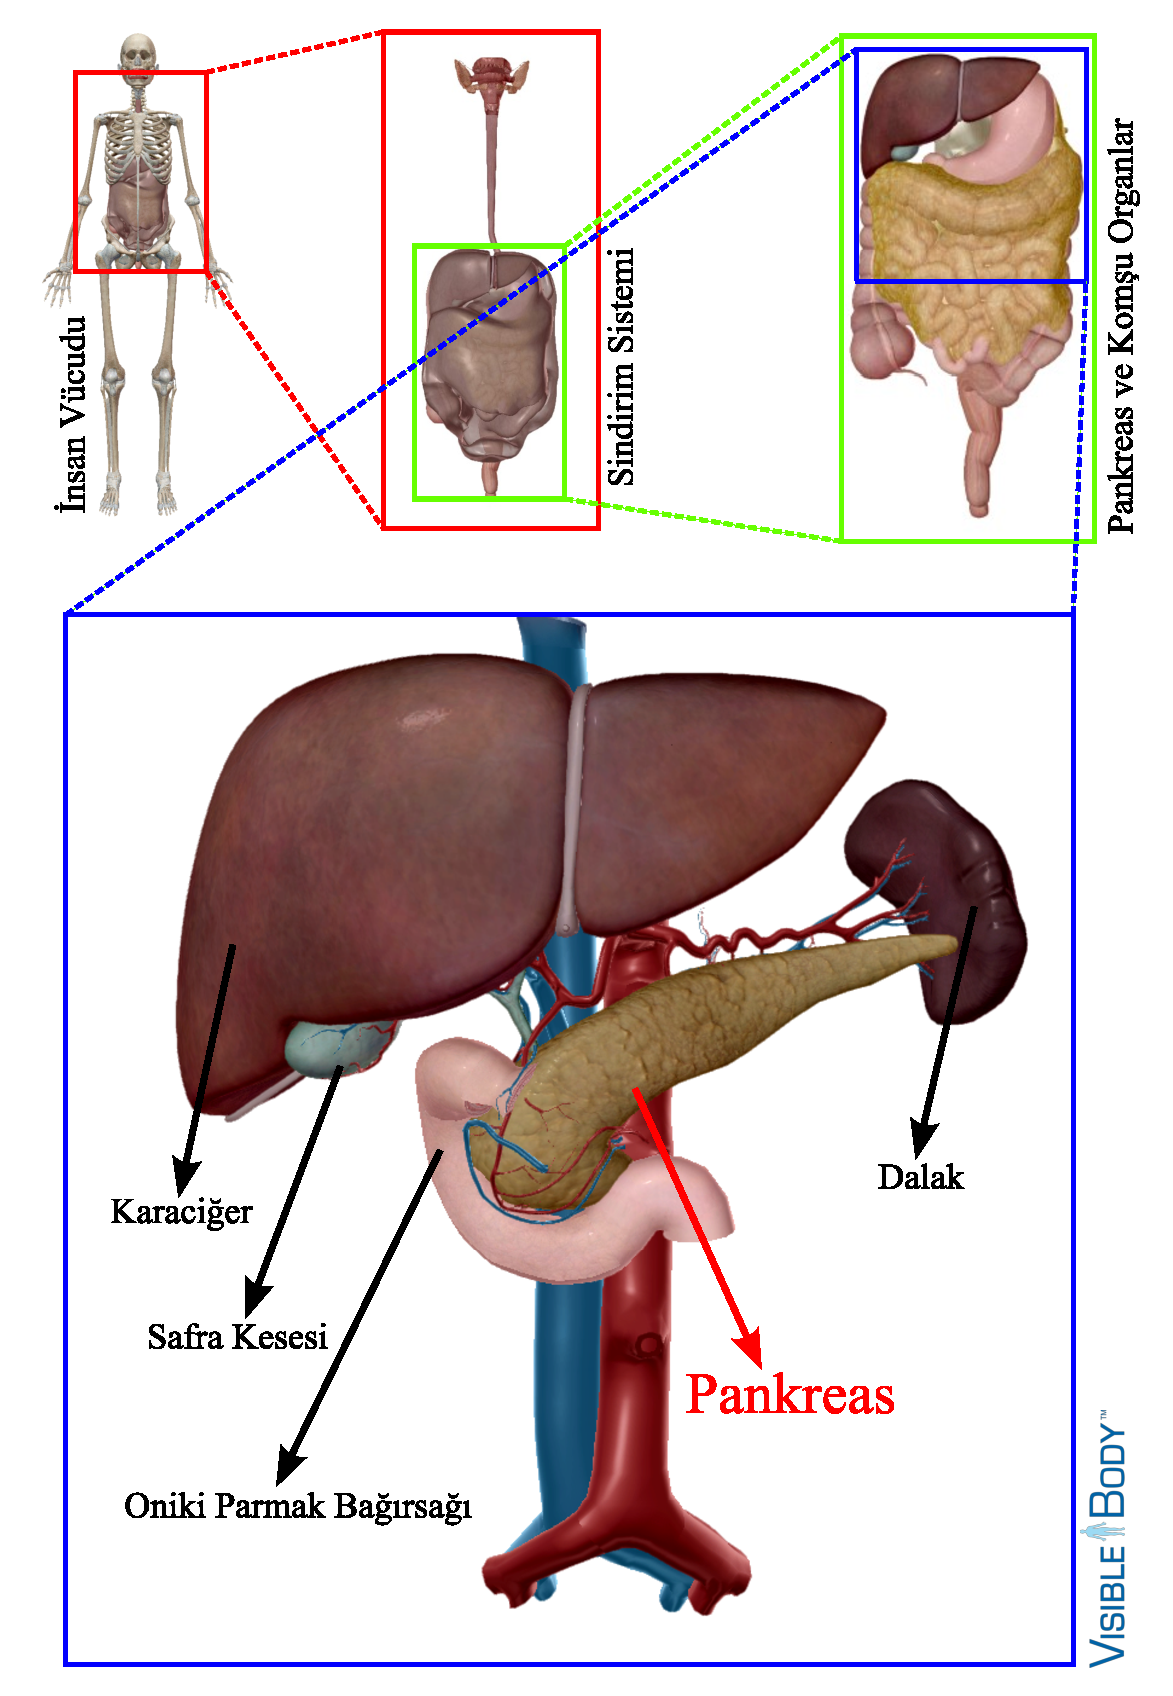
\includegraphics[scale=0.66]{Genel-Bilgiler/Figures/pankreas_location.pdf}
		}
	\end{center}
\end{figure}

Pankreas organının vücudumuzda oldukça önemli iki ana işlevi bulunmaktadır. Bunlar sindirime yardımcı olan sindirim enzimlerinin üretilmesinde rol alan ekzokrin işlevi ve kan şekerini düzenleyen insülin, glukagon gibi hormonların salgılanmasını sağlayan endokrin işlevidir [3-5]. Ekzokrin ve endokrin işlevleri şu şekilde açıklanabilmektedir:

-  Ekzokrin İşlevi:

Şekil \ref{fig:pank_ekzokrin}’te görüldüğü gibi pankreas organı, sindirim için önemli enzimler üreten ekzokrin bezleri içermektedir. Bu enzimlerin görevi ve isimleri sırasıyla şu şekildedir: protein sindirmek için tripsin ve kimotripsin; karbonhidratların sindirimi için amilaz; ve yağları parçalamak için lipaz. Yiyecek mideye ulaştığı zaman, pankreas özsuları ana pankreas kanalına ulaşan kanal sistemine salınmaktadır. Pankreas kanalı, duodenum adı verilen ince bağırsağın ilk kısmında yer alan Vater ampullasını oluşturmak için ortak safra kanalına katılmaktadır. Ortak safra kanalı, karaciğer ve safra kesesinden oluşmakta olup safra adı verilen bir başka önemli sindirim suyu üretmektedir. Oniki parmak bağırsağına salınan pankreas özsuları ve safra, vücudun yağları, karbonhidratları ve proteinleri sindirmesine yardımcı olmaktadır.

\captionsetup[figure]{margin={0.3cm,0cm}}
\begin{figure}[h!]
	\begin{center}
		\vspace{0.4cm}
		\captionbox{Pankreas organının Ekzokrin işlevi \cite{pancreaslocationimage}.
			\label{fig:pank_ekzokrin}}
		{
			\vspace{0.4cm}
			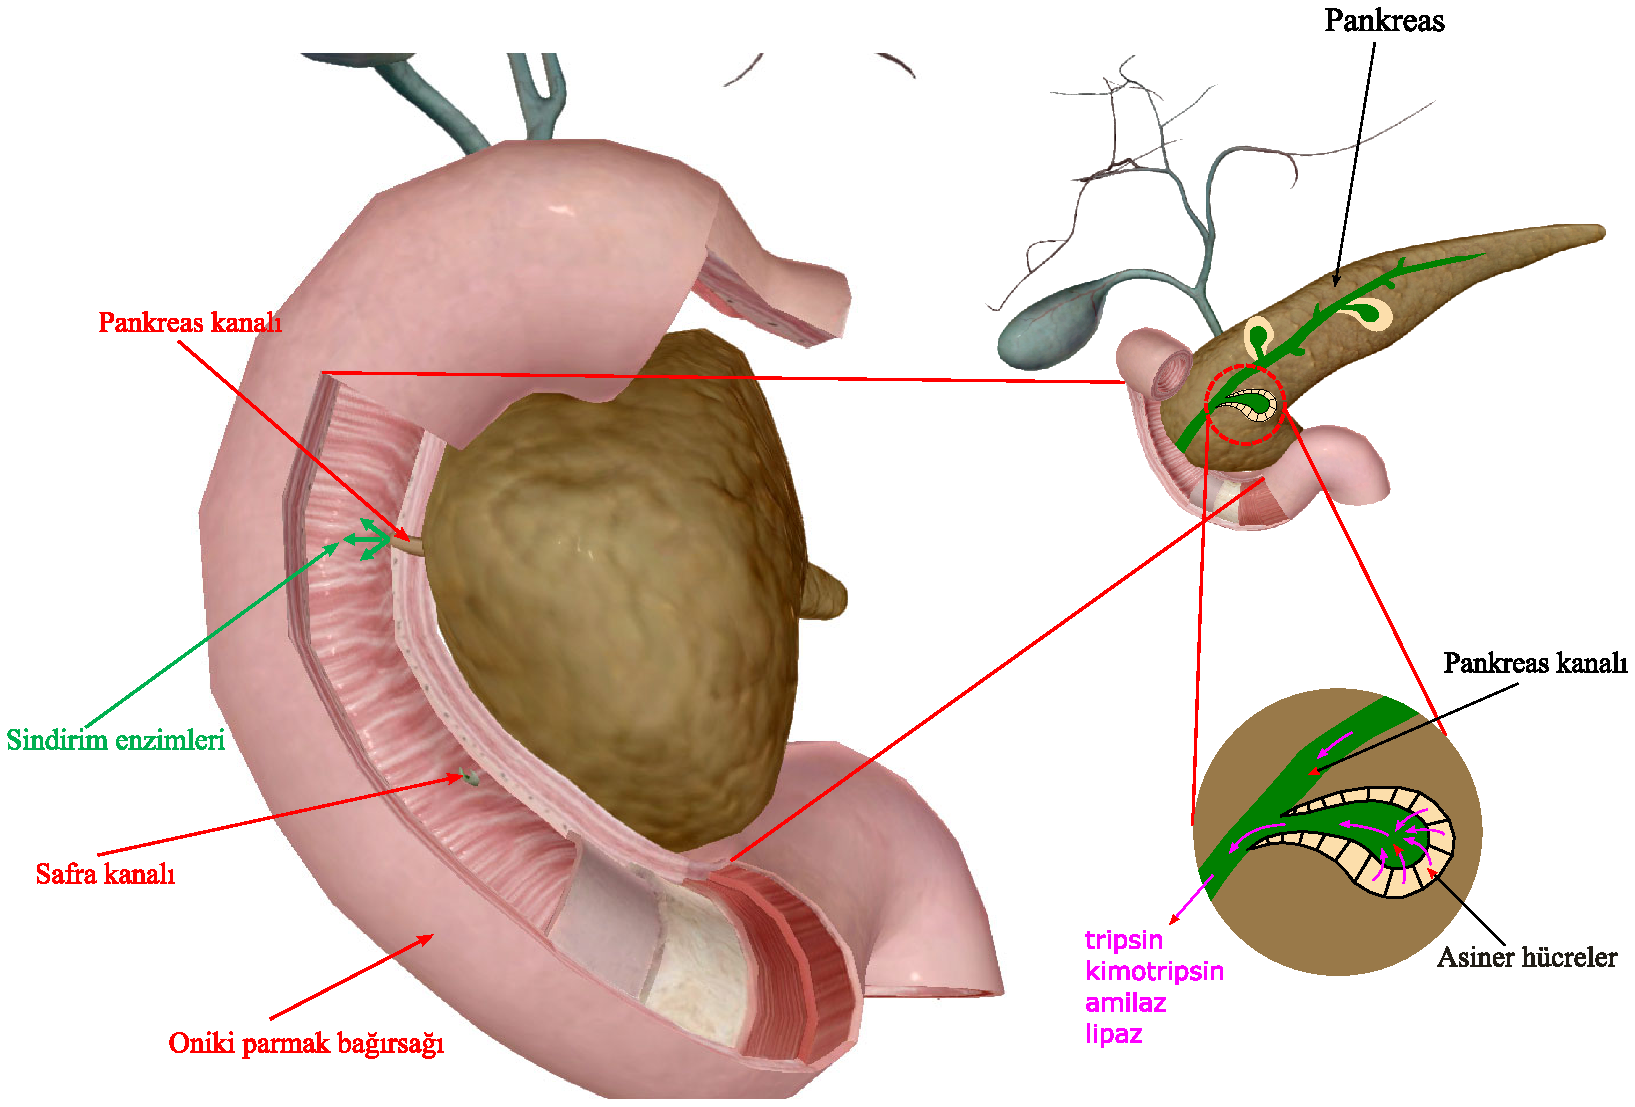
\includegraphics[scale=0.55]{Genel-Bilgiler/Figures/ekzokrin_function.pdf}
		}
	\end{center}
\end{figure}

- Endokrin İşlevi:

Pankreasın endokrin bileşeni, Şekil \ref{fig:pank_endokrin}’te görüldüğü gibi önemli hormonları oluşturan ve doğrudan kan dolaşımına salan adacık hücrelerinden oluşmaktadır. Adacık hücrelerinin yaklaşık \%70'i beta hücrelerinden, \%20'si alfa hücrelerinden ve \%10'u delta hücrelerinden oluşmaktadır. Bu hücrelerden beta hücreleri insülin, amilin hormonlarını, alfa hücreleri glukagon hormonunu, Delta hücreleri ise somatostatin hormonunu üreterek damarlar vasıtası ile kana iletilmektedir \cite{krahl1974endocrine}. Bu hormonların en önemli görevi kan şekerini dengelemektir.  Uygun kan şekeri seviyelerini korumak, beyin, karaciğer ve böbrekler dahil olmak üzere kilit organların işleyişi için çok önemlidir.


\captionsetup[figure]{margin={0.4cm,0cm}}
\begin{figure}[h!]
	\begin{center}
		\vspace{0.4cm}
		\captionbox{Pankreas organının Endokrin işlevi \cite{pancreaslocationimage}.
			\label{fig:pank_endokrin}}
		{
			\vspace{0.4cm}
			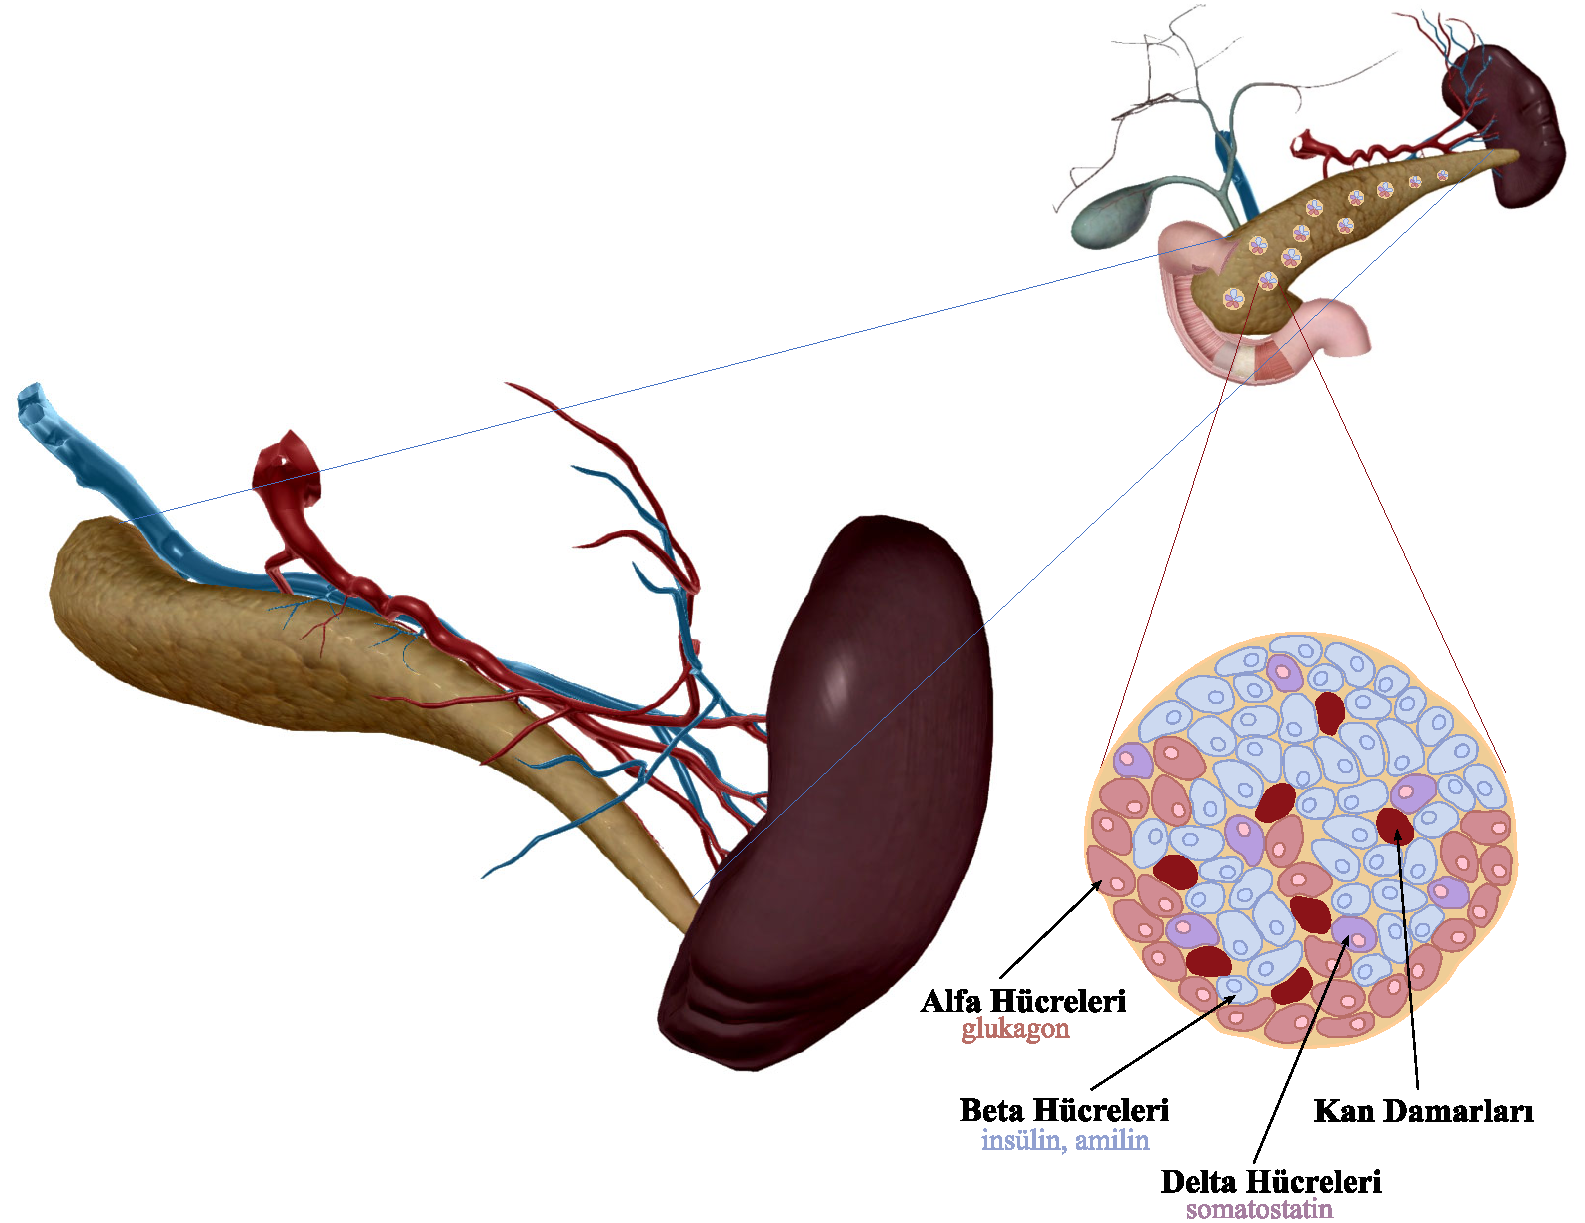
\includegraphics[scale=0.57]{Genel-Bilgiler/Figures/endokrin_function.pdf}
		}
	\end{center}
\end{figure}

\section{Pankreas ve Pankreas Kanseri Görüntüleme Teknikleri}

Günümüzde pankreas kanseri tanısı, tümörlü dokuların konumunun tespiti ve hastalığın evrelendirilebilmesi gibi amaçlar için Ultrason, Endoskopik Ultrason (EUS), Bilgisayarlı Tomografi (BT), Manyetik Rezonans (MR), Endoskopik Retrograd Kolanjiopankreatografi (ERCP), İnce İğne Aspirasyonu gibi teknikler ön plana çıkmaktadır \cite{goral2014pankreas,freelove2006pancreatic,cameron2001pancreatic,chu2017diagnosis}.

Görüntüleme tekniğinin hasta bireylerin tanılanmasında gösterdiği başarı Duyarlılık olarak adlandırılmaktadır. Yine ilgili görüntüleme tekniğinin sağlıklı bireylere tanı koymada gösterdiği başarıya da Özgüllük denilmektedir. Görüntüleme tekniklerinin bir hastalığa tanı konmasında kullanılabilmesi için ilgili testin Özgüllük (\%) ve Duyarlılık (\%) değerlerinin toplamının 170 değerinden büyük olması beklenmektedir. Ayrıca pankreas kanseri gibi kanser dokularının oluşturduğu tümörlü bölgenin ebatları ve konumu hastalığın evrelenmesinde önemli rol oynamaktadır. Bu sebeple pankreas kanserine tanı konmasında kullanılacak görüntüleme tekniğinin Duyarlılık ve Özgüllük metriklerinin dışında hastalığın evrelendirilmesindeki başarısı da önem arz etmektedir.

\begin{table}[h!]	
	\caption{Pankreas kanseri tanı ve evrelendirmesinde kullanılan başlıca görüntüleme yöntemleri.\cite{goral2014pankreas}}
	\begin{tabular}{m{6cm}m{2.5cm}m{2.5cm}m{3cm}}
		& \textbf{Özgüllük} & \textbf{Duyarlılık} & \textbf{Evrelemede Fayda} \\ \hline
		Ultrason                                              & 80\%     & 90\%       & YOK                   \\ \hline
		Endoskopik Ultrason (EUS)                             & 90\%     & 90\%       & VAR                   \\ \hline
		Endoskopik Retrograd Kolanjiopankreotografi (ERCP) & 90\%     & 90\%       & YOK                   \\ \hline		
		İnce İğne Aspirasyonu                                 & 90\%     & 98\%       & YOK 
		\\ \hline
		Magnetik Rezonans (MR)                                & 90\%     & 90\%       & YOK                   \\ \hline
		\rowcolor{Gray}
		Bilgisayarlı Tomografi (BT)                           & 90\%     & 95\%       & VAR                                    
	\end{tabular}
	\label{tab:goruntulemeteknikleri}
\end{table} 

Tablo \ref{tab:goruntulemeteknikleri}'de görüldüğü gibi BT görüntüleme pankreas kanserini evreleme aşamasında en fayda sağlayan görüntüleme tekniğidir. Bu teknik en yüksek Özgüllük ve Duyarlılık seviyelerine sahip olan görüntüleme tekniği olarak ön plana çıkmaktadır. Dolayısıyla pankreas kanserine tanı konması ve evrelendirilmesi için çoğunlukla BT görüntüleme tekniği tercih edilmektedir.

\subsection{Ultrason}

Ultrason pankreas kanseri belirtilerinden olan karın ağrısı ve sarılık gibi durumlarla karşılaşıldığında daha uygun maliyetli olması ve insan sağlığına daha az zararlı olması gibi sebeplerden dolayı öncelikle tercih edilen görüntüleme tekniği olarak karşımıza çıkmaktadır \cite{wells2006ultrasound,chan2011basics,sofuni2005differential}. Ultrasonun çalışma prensibi yüksek frekanslı ses dalgalarının farklı dokulardan farklı miktarlarda yansıma yapmasına dayalıdır. Ultrason cihazını kullanan operatörün yetenekleri ve bağırsak gazlarının pankreas dokusunu maskelemesi gibi durumlar bu görüntüleme tekniğinin Özgüllük ve Duyarlılığını fazlasıyla etkilemektedir. Bu sebeple genellikle ilk teşhisin koyulmasında kullanılmakta sonrasında ise daha gelişmiş görüntüleme tekniklerine ihtiyaç duyulmaktadır.

\subsection{Endoskopik Ultrason (EUS)}

Bu görüntüleme tekniği, endoskopik yoldan sindirim sistemini oluşturan yemek borusu, mide, pankreas, karaciğer, safra kesesi ve bağırsaklar gibi organlarda ortaya çıkabilen kitle ve lezyonların tanı, teşhis ve evrelendirilmesinde sıklıkla kullanılmaktadır. Endoskopik yoldan salınan esnek kablo ucundan yüksek frekanslı ses dalgaları gönderilerek endoskopik yol etrafındaki farklı yoğunluklu organlardan yansıyan ses dalgaları kullanılması prensibine dayalı bir görüntüleme tekniğidir. Ultrasona göre çok daha hassas bir görüntüleme sağlayabilmektedir. Pankreas kanserinin ve tümörlü dokuların ilk teşhisinde sıklıkla tercih edilmektedir\cite{rosch1991endoscopic,anderson2000endoscopic}. Ultrasonda olduğu gibi cihazı kullanan operatörün yetenekleri ve ilgili bölgedeki bağırsak gazı yoğunluğu bu görüntüleme tekniğinin Özgüllük ve Duyarlılığını fazlasıyla etkilemektedir.

\subsection{Endoskopik Retrograd Kolanjiopankreatografi (ERCP)}	

Bu görüntüleme tekniğinde endoskopik yoldan ucunda ışıklı kamera bulunan özel bir endoskopi cihazı ile yemek borusu üzerinden mideye ve mideden de oniki parmak bağırsağına ulaşılmaktadır. Oniki parmak bağırsağına bağlanan milimetrik boyutlardaki safra kanalı üzerinden de ince uçlu kateter denilen cihazlarla safra kanalına yada pankreas kanalına kontrast madde enjekte edilmektedir. Daha sonra x ışınları kullanan bir cihaz ile enjekte edilen kontrast maddenin ilgili dokularda görüntülenmesi sağlanarak taş ve tümör gibi anormalliklerin teşhisi sağlanmaktadır \cite{oi1998ercp,hanada2019roles}. Kontrast maddenin direk hedef bölgeye uygulanmasından dolayı daha kullanışlı sonuçlar elde edilebilmektedir. Bu işlem genel olarak güvenli olmakla beraber bazı istenmeyen yan etkilerle karşılaşılabilmektedir \cite{mallery2003complications}. Özellikle pankreas tümörlerinin tespitinde kullanıldığında pankreas bezlerinin iltihaplanması (pankreatik) durumu ile karşılaşılabilmekte ve tümör evrelemede yeterli görülmemektedir.

\subsection{İnce İğne Aspirasyonu}

Bu teknikte ince uçlu bir iğne ile kanser şüphesi bulunan kitlelere genellikle endoskopik ultrason rehberliği ile ulaşılarak doku örneği alınmaktadır \cite{robins1995fine,harewood2002endosonography,frossard2003performance}. Öncelikle vücudun dışından iğne ile giriş yapılacak bölge lokal olarak uyuşturulmaktadır. Daha sonra lokal uyuşturulan bu bölgeden girilerek hedef kitleye ulaşılmaktadır. Bu teknikle elde edilen doku örnekleri incelenelerek kitlenin türüne göre tanı ve tedavi prosedürleri uygulanabilmektedir. Genellikle işlem bir sitopatalog eşliğinde yapılmaktadır. Sitapatoloğun mesleki deneyimi alınan doku örneklerine tanı konmasında yeterli olması oldukça önemlidir. Bu yöntemde kitle bütünlüğü ve pankreasa komşu organlarla ilişkisi görüntülenemediği için hastalığı evrelemede fayda sağlamamaktadır. 

\subsection{Manyetik Rezonans (MR)}

İnsan vücudundaki organ ve dokuların, radyo dalgaları ve manyetik alanların kullanılmasıyla detaylı ve yüksek çözünürlüklü görüntülenebilmesi için kullanılan bir görüntüleme tekniğidir \cite{reimer2010clinical,semelka1993mr,tirkes2012mr}. Bilgisayarlı Tomografi görüntüleme tekniğinin aksine x-ray ışınları ve iyonize radyasyon içermediği için insan sağlığına çok daha az zararlıdır. MR genellikle beyin omurilik hastalıkları, kas yaralanmaları ve nörolojik hastalıkların teşhisinde tercih edilmektedir. Bazı özel durumlarda pankreas tümörü tespitinde başarılı sonuçlar verebilmektedir. Fakat genellikle pankreas kanseri evreleme aşamasında yeterli görülmemektedir. Kalbinde pil yada stent takılı, dişlerinde tel takılı yada vücudunda herhangi çelik içerikli protez bulunan hastalarda manyetik çekim gücünün sebep verebileceği hasarlardan dolayı kullanılamamaktadır.

\subsection{Bilgisayarlı Tomografi (BT)} 

Bilgisayarlı tomografi (BT) insan vücudunun, organlarının, iskelet sisteminin ve diğer dokuların detaylı volumetrik görüntülerinin oluşturulması için x-ışınlarının kullanıldığı radyolojik bir görüntüleme tekniğidir. Bilgisayarlı tomografi cihazları temelde hastanın üzerinde uzandığı yatay eksende hareketli tabya, tabya etrafında dairesel dönen x-ışını üretici ve yine tabya etrafında dönen ve x-ışını üreticinin karşısına konumlandırılmış x-ışını dedektöründen oluşmaktadır \cite{kalender2011computed,seeram2015computed}. X-ışını üreticisinden üretilen ışınlar hasta vücudundaki farklı yoğunluklu dokulardan geçerken farklı miktarda zayıflamaya maruz kalarak x-ışını dedektörü tarafından yakalanmaktadırlar. Şekil \ref{fig:ct_block}'da bilgisayarlı tomografi (BT) cihazının çalışma prensibi görselleştirilmektedir. Burada da görüldüğü gibi x-ışını dedektörü tarafından algılanan farklı miktarlarda zayıflamaya uğramış x-ışınları işlenerek yatay vücut kesit görüntüleri elde edilmektedir. 

\captionsetup[figure]{margin={0.4cm,0cm}}
\begin{figure}[h!]
	\begin{center}
		\vspace{0.4cm}
		\captionbox{Bilgisayarlı tomografi (BT) cihazının çalışma prensibi.
			\label{fig:ct_block}}
		{
			\vspace{0.4cm}
			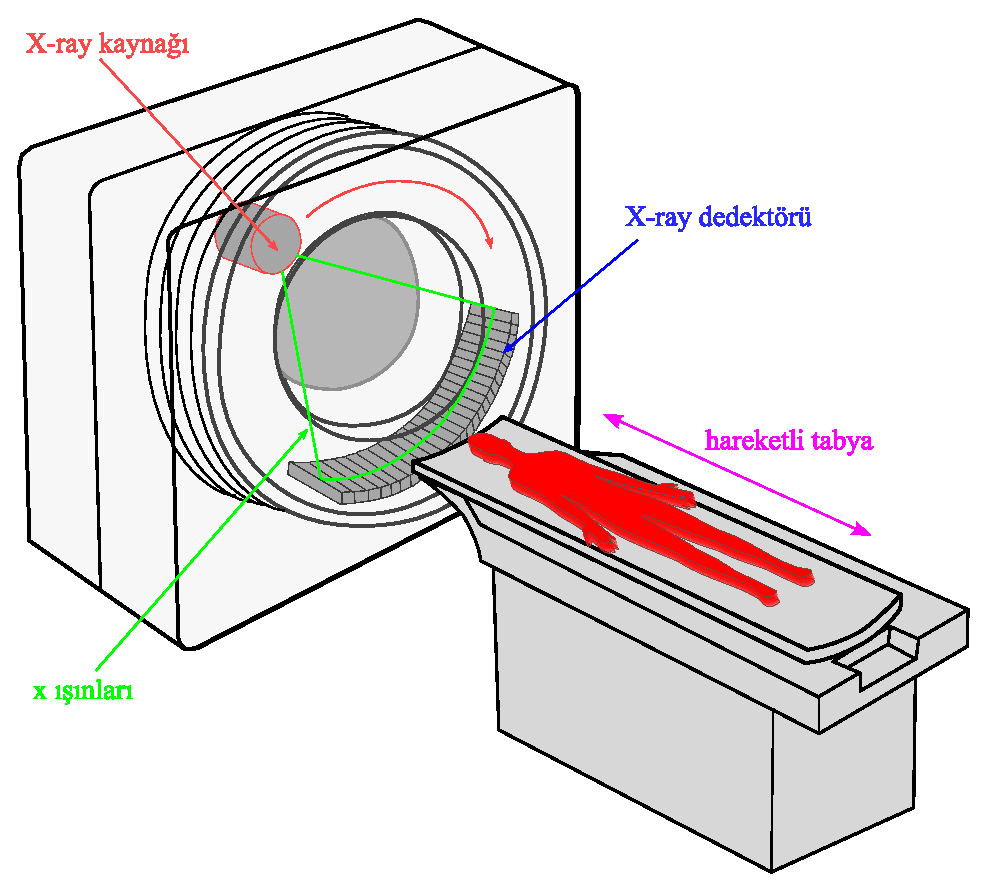
\includegraphics[scale=0.68]{Genel-Bilgiler/Figures/ct_block.pdf}
		}
	\end{center}
\end{figure}

Sıralı elde edilen bu kesit görüntüleri birleştirilerek volumetrik vücut verisi üretilmektedir. Bu volumetrik verideki her 3B piksel voksel olarak adlandırılmaktadır. Piksel ifadesi matris boyutu ve görüş alanına bağlı iki boyutlu bir birimken, BT diliminin kalınlığı da dikkate alındığında bilgisayarlı tomografi görüntüleme tekniğindeki üç boyutlu bir birim olan voksel terimi tercih edilmektedir. Volumetrik BT taramasındaki her bir dilimin üretilmesinde Şekil \ref{fig:ct_hounsfield}'de gösterilen ve Hounsfield ölçeği denilen bir ölçeklendirme tekniği kullanılmaktadır. Hounsfield ölçeğinde x-ışınlarında en çok zayıflamaya sebep veren dokuların voksel değeri +3071 ile temsil edilirken en az zayıflamaya sebep olan dokuların voksel değeri ise -1024 ile temsil edilmektedir \cite{hounsfield1973computerized}.

\captionsetup[figure]{margin={0.5cm,0cm}}
\begin{figure}[h!]
	\begin{center}
		\vspace{0.4cm}
		\captionbox{Bilgisayarlı tomografi (BT) Hounsfield ölçeği ile volumetrik veri elde edilmesi.
			\label{fig:ct_hounsfield}}
		{
			\vspace{0.4cm}
			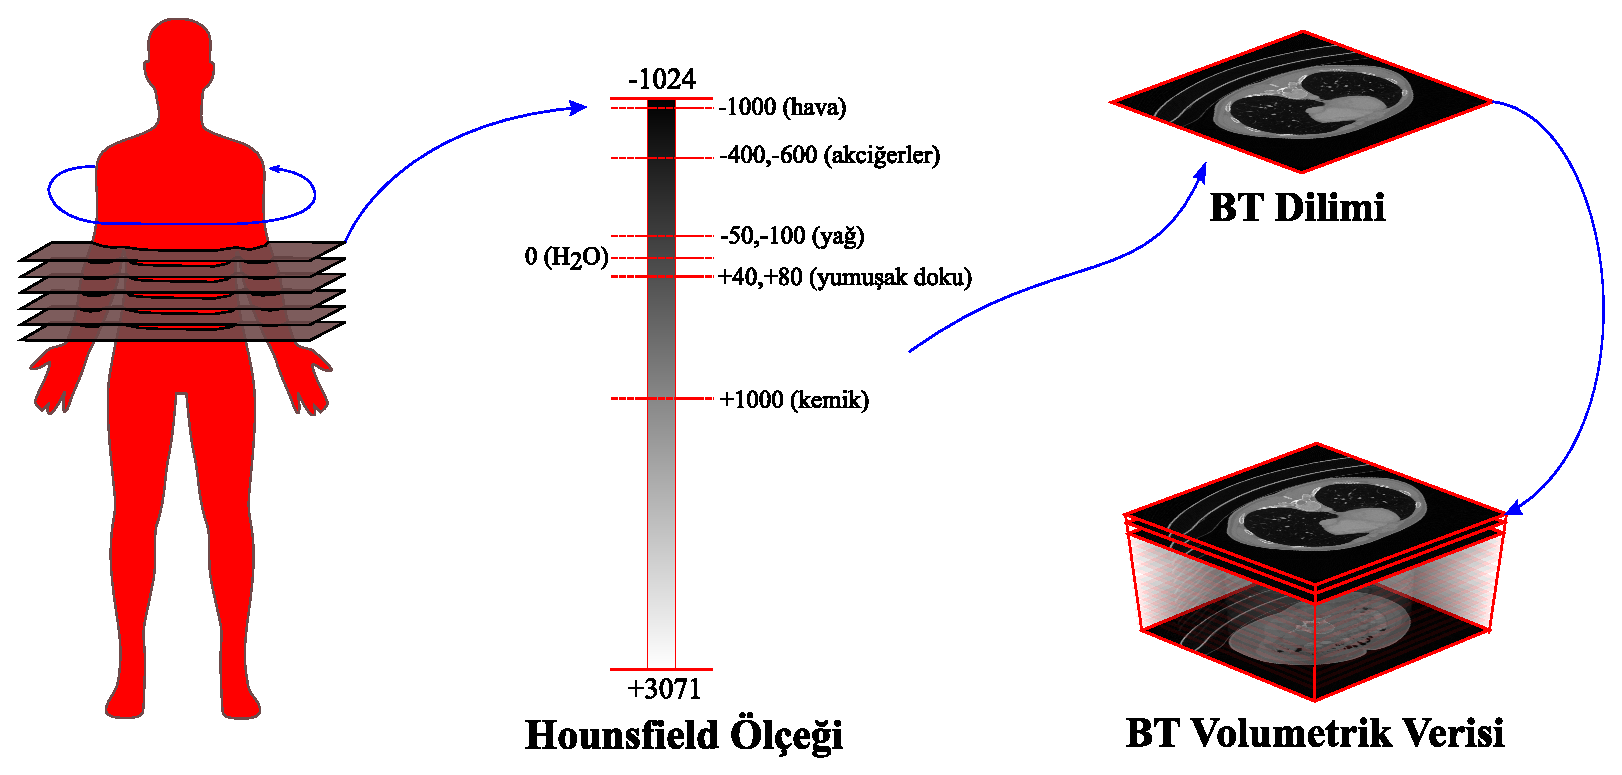
\includegraphics[scale=0.55]{Genel-Bilgiler/Figures/ct_hounsfield.pdf}
		}
	\end{center}
\end{figure}

Bilgisayarlı tomografi görüntüleme tekniği yaralanma, kalp hastalıkları, kemik, eklem ve doku zedelenmesi, organlar ve organlarda ortaya çıkan kitleler gibi anomalilerin tespiti, zatürre gibi akciğer hastalıklarının tespiti gibi çok çeşitli alanlarda doktorlara müdahale öncesinde önemli ön bilgiler sunabilmektedir. Özellikle pankreas hastalıkları ve pankreas kitlelerinin detaylı incelemelerinde sıklıkla tercih edilmektedir. Tablo \ref{tab:goruntulemeteknikleri}'de görüldüğü gibi diğer görüntüleme tekniklerine göre daha üstün tanılama bilgileri sağlamaktadır. Bu sebeple pankreas organının zor konumu ve fizyolojik yapısı düşünüldüğünde bilgisayarlı tomografi oldukça kritik bir görüntüleme tekniği olarak karşımıza çıkmaktadır. 

İnsan vücudu anatomik olarak incelendiğinde pankreas organı head, thorax, abdomen ve pelvis gibi bölgelerden abdomen bölgesinde yer almaktadır. Bu sebeple pankreas hastalıkları için bilgisayarlı tomografi görüntüleme tekniği kullanıldığında abdomen bölgesi için tarama gerçekleştirilmektedir. Pankreastaki kitlelerin bilgisayar destekli tanılama sistemlerince işlenebilmesi amacıyla abdomen bölgeden volumetrik görüntüler alınmaktadır. Volumetrik bilgisayarlı tomografi görüntülerinin her biri uzman kişilerce pankreas ve tümör dokularının bulunduğu bölgelerin işaretlenmesi için incelenmektedir. Bu sayede Şekil \ref{fig:pancreas_abdomen}'deki gibi veri setleri üretilebilmektedir. 

\captionsetup[figure]{margin={0.3cm,-1cm}}
\begin{figure}[h!]
	\begin{center}
		\vspace{0.4cm}
		\captionbox{Abdomen bölgeden elde edilen volumetrik BT verisinin manuel olarak işaretlenmesi ile oluşturulan pankreas bölgesi \cite{pancreaslocationimage}.
			\label{fig:pancreas_abdomen}}
		{
			\vspace{0.4cm}
			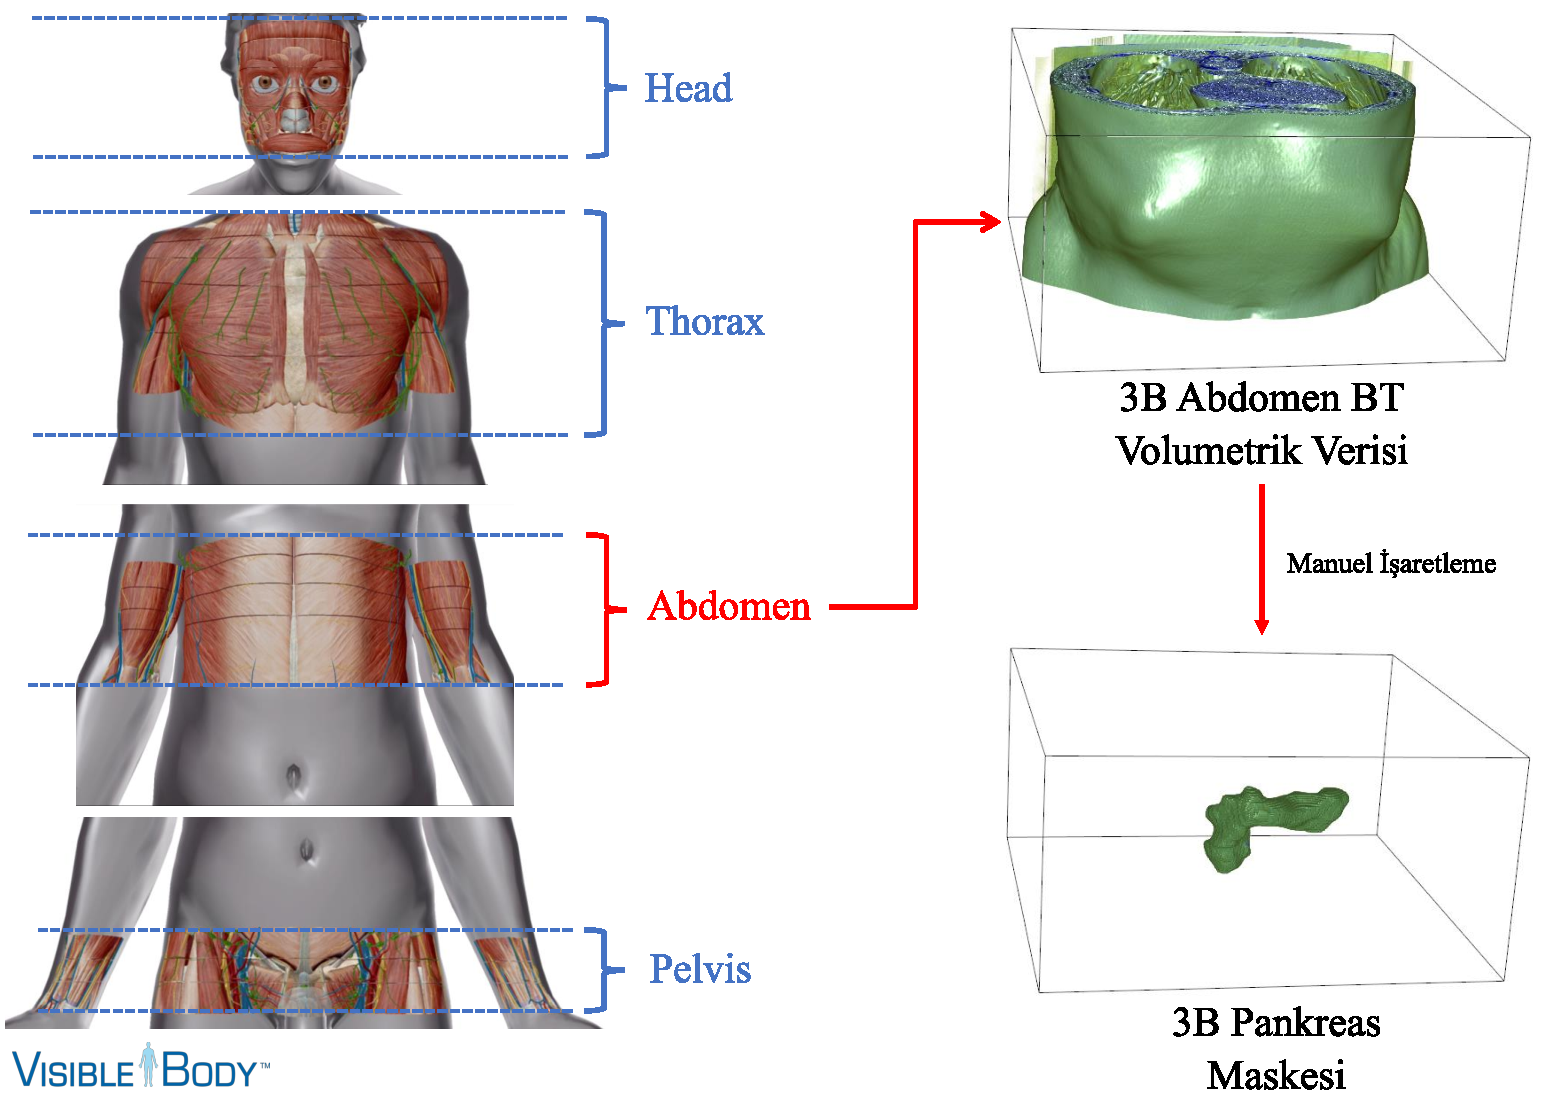
\includegraphics[scale=0.5]{Genel-Bilgiler/Figures/pancreas_abdomen.pdf}
		}
	\end{center}
\end{figure}

\section{Tez Çalışmasında Kullanılan Veri Setleri}
Tez çalışmamızda literatürdeki çalışmalara göre BT görüntülemede daha yüksek doğrululuğa sahip otomatik pankreas ve pankreas tümörü segmentasyonu sağlamak amaçlanmaktadır. Bu kapsamda pankreas ve pankreas tümör segmentasyonu için CNN tabanlı yaklaşımlar geliştirilmektedir. 

Tez çalışmasının ilk kısmında pankreas segmentasyonu için ilgi bölgesi belirlenerek bölge küçültme tekniği ile çalışan bir yöntem önerilmektedir. Önerilen yöntemde veri setinin iki sınıflı (pankreas, diğer dokular) olması, kanser dokularının segmentasyonunu içermemesi ve daha basit işlenebilir olmasından dolayı Ulusal Sağlık Enstitüleri Pankreas BT Veri Seti (National Institutes of Health Clinical Center Pancreas CT - NIH Pancreas CT) kullanılmaktadır.

Tez çalışmasının ikinci kısmında pankreas ve pankreas tümörü segmentasyonu için CNN tabanlı yaklaşımlar önerilmektedir. İkinci kısımda pankreas kanser dokularının da işaretli olduğu üç sınıflı (pankreas, pankreas tümörü, diğer dokular) bir veri setinde önerilen yöntemin farklı segmentasyon teknikleri ile performansının incelenmesi hedeflenmektedir. Bu amaçla tezin ikinci kısmında Tıbbi Segmentasyon Dekatlon Veri Seti (Medical Segmentation Decathlon - MSD) kullanılmaktadır.

\subsection{Ulusal Sağlık Enstitüleri Pankreas BT Veri Seti (National Institutes of Health Clinical Center Pancreas CT - NIH Pancreas CT)}

Pankreas segmentasyonu için Konvolüsyonel Sinir Ağlarına dayanan ilk çalışma Roth tarafından geliştirilmiş ve bu çalışmada NIH pankreas veri seti oluşturulmuştur \cite{roth2015deep}. Yapılan tez çalışmasının ilk kısmı olan pankreas segmentasyonu için önerilen iki aşamalı yaklaşımı değerlendirmek için NIH pankreas veri seti kullanılmaktadır. Bu veri setindeki BT görüntüleri DICOM formatında kaydedilmiştir.

\captionsetup[figure]{margin={0.2cm,0cm}}
\begin{figure}[h!]
	\begin{center}
		\vspace{0.4cm}
		\captionbox{NIH pankreas veri setine ait örnek 2B BT dilimleri ile 2B BT dilimlerinin manuel olarak etiketlenmiş ikili maskeleri.\label{fig:nih_2dslices}}
		{
			\vspace{0.4cm}
			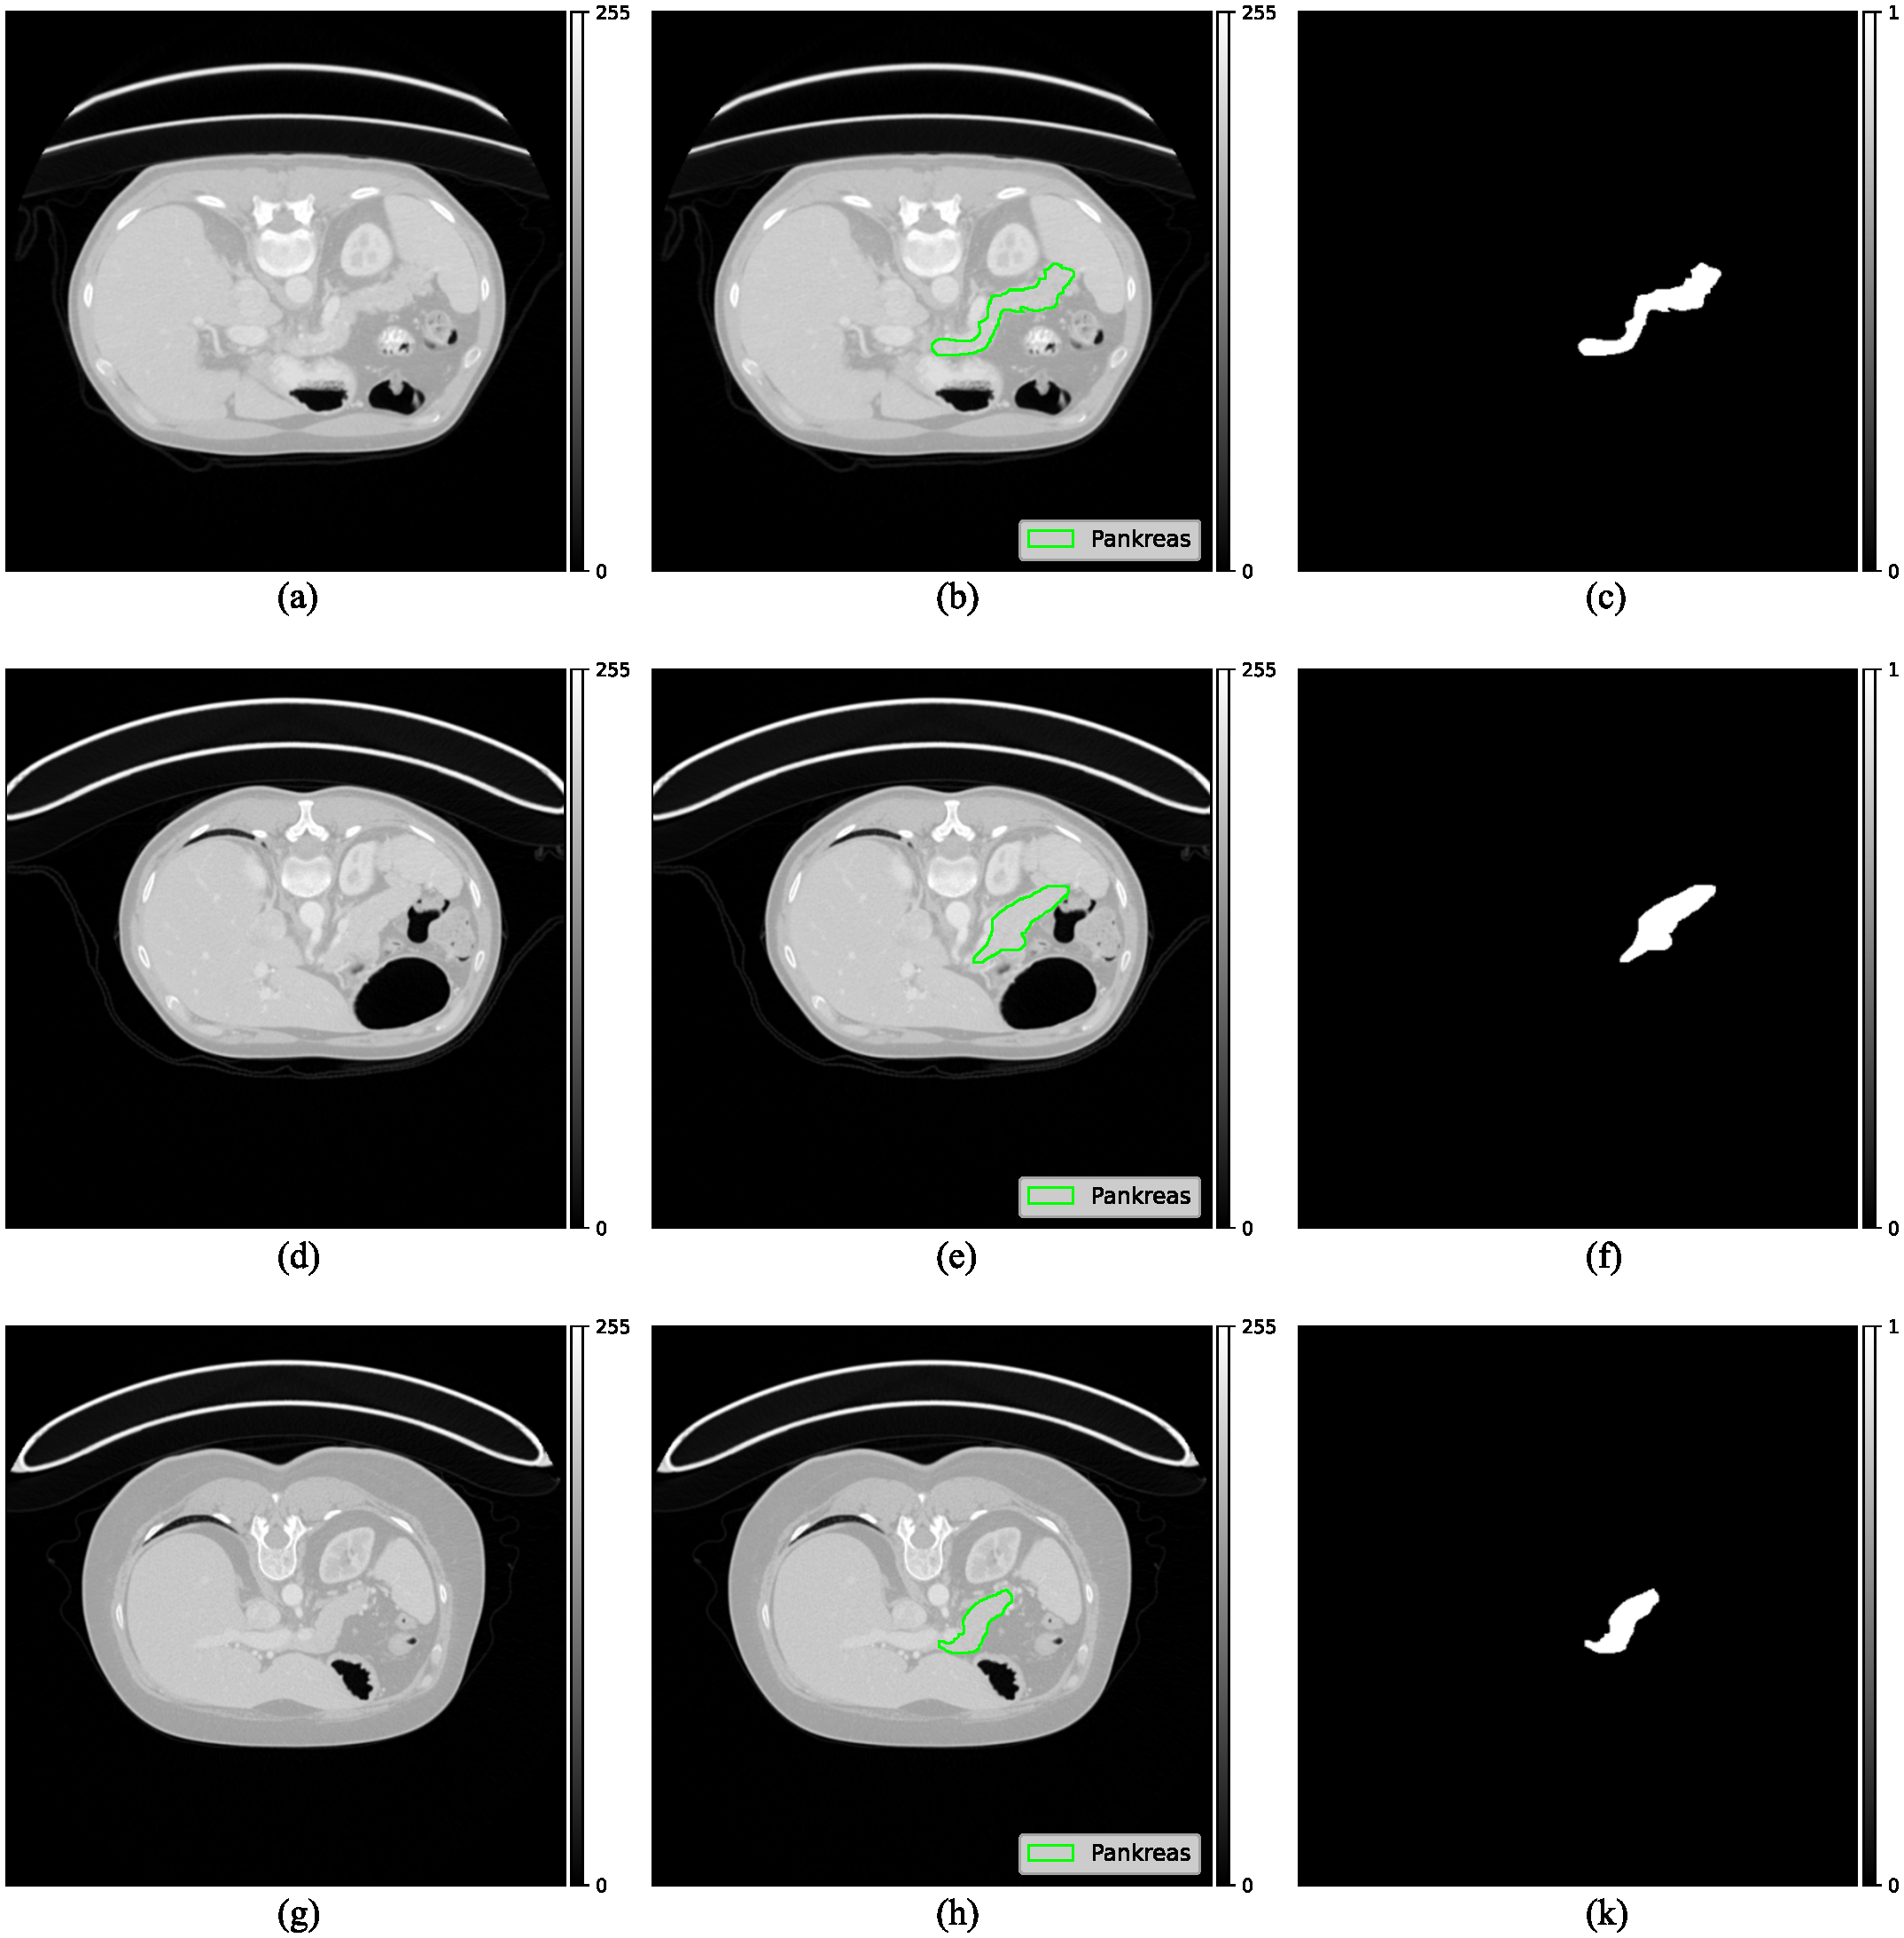
\includegraphics[scale=0.42]{Yapilan-Calismalar/Figures/nih_2dslices.pdf}
		}
	\end{center}
\end{figure} 

NIH veri setinde $82$ abdominal kontrastlı BT taraması ve ilgili taramalara ait BT dilimlerinin ayrı ayrı manuel olarak pankreas bölgeleri işaretlenmiş ikili (pankreas, diğer dokular) maskeleri bulunmaktadır. Her BT taramasındaki görüntülerin boyutu $512 \times 512 \times N$’dir. Burada $N$, BT taramalarındaki dilim sayısını ifade etmektedir. Veri setinde $N$ sayısı $181$ ile $466$ arasında değişmektedir. Veri seti oluşturulurken seçilen dilim kalınlığı $1,5$ mm ile $2,5$ mm arasında değişmektedir. Şekil \ref{fig:nih_2dslices}’da NIH pankreas veri setine ait bazı 2B görüntüler ile bu görüntülerin manuel olarak etiketlenmiş ikili maskeleri gösterilmektedir. BT taramalarındaki pankreas sınırları uzman doktorlar tarafından işaretlenmiştir. 

Tez çalışmasının ilk kısmında Pankreas İlgi Bölgesinin Belirlenmesi ve Pankreas Segmentasyonu fazlarının test ve eğitimi için NIH veri seti \%80 eğitim ve \%20 test olmak üzere iki parçaya ayrılmaktadır. Ayrıca, eğitim seti 4 rastgele gruba ayrılmakta ve 4-kat çapraz doğrulama gerçekleştirilmektedir. Üç set alt eğitim için, bir set ise validasyon için kullanılmaktadır. Alt eğitim ve validasyon seti, derin ağlarda parametre ayarlaması yapmak için kullanılmaktadır. En iyi ağ, sinir ağının eğitimi sırasında gerçekleştirilen validasyon ile elde edilen doğruluk ve hataya bağlı olarak belirlenmektedir. Ardından, önerilen ağının performansı test seti üzerinde ölçülmektedir.

\subsection{Tıbbi Bölütleme Dekatlon Veri Seti (Medical Segmentation Decathlon - MSD)}

Yapılan tez çalışmasının ikinci kısmında ilk kısımda önerilen iki aşamalı yöntemin 3 sınıflı (pankreas, pankreas tümörü, diğer dokular) kanser dokularının bulunduğu daha kompleks bir veri setinde performansı incelenmektedir. Bu kapsamda tez çalışmasının ikinci kısmında Tıbbi Bölümleme Decathlon Veri Seti (Medical Segmentation Decathlon - MSD) kullanılmaktadır. Bu veri seti  2018 yılında İspanya, Granada'daki Tıbbi Görüntü Hesaplama ve Bilgisayar Destekli Müdahaleler Konferansı (Medical Image Computing and Computer Aided Interventions Conference - MICCAI) sırasında kullanılmıştır \cite{simpson2019large}. 

BT taramalarındaki görüntüler Memorial Sloan Kettering Kanser Merkezi (New York, NY, ABD) tarafından sağlanmış ve daha önce radyomik uygulamalarda kullanılmıştır \cite{attiyeh2018survival,attiyeh2019preoperative,chakraborty2018ct}. Bu veri setindeki BT dilimleri DICOM formatında kaydedilmiştir. Bu veri setinde, kanserli organ segmentasyonu için kullanılabilecek $10$ farklı abdominal organdan çekilmiş BT taramaları mevcuttur. Bu organlar sırasıyla kalp, akciğer, hipokampus, prostat, akciğer, damar, dalak ve kolondur. Tez çalışması kapsamında gerçekleştirilen yaklaşımların değerlendirilmesi için MSD veri setinin pankreas ve pankreas tümörünü kapsayan alt veri seti kullanılmıştır. 

Pankreas veri seti, pankreas kitlelerinin (intraduktal müsinöz neoplazmalar, pankreas nöroendokrin tümörleri veya pankreas duktal adenokarsinomu) rezeksiyonu uygulanan hastalardan elde edilen BT taramalarından oluşmaktadır. Veri setinde $281$ abdominal kontrastlı BT taraması ve ilgili taramalara ait etiketler ile oluşturulmuş ikili maskeler bulunmaktadır. Her BT taramasındaki görüntülerin boyutu $512 \times 512 \times N$’dir. Burada $N$, BT taramalarındaki dilim sayısını ifade etmektedir. Veri seti oluşturulurken dilim kalınlığı $2,5$ mm olarak alınmaktadır. Şekil \ref{fig:msd_2dslices}’da Tıbbi Bölümleme Decathlon veri setine ait bazı 2B görüntüler ile bu görüntülerin manuel olarak etiketlenmiş ikili maskeleri gösterilmektedir. BT taramalarındaki pankreas sınırları uzman doktorlar tarafından işaretlenmiştir. Pankreas parankimi ve pankreas kitlesi (kist veya tümör), Scout uygulaması kullanılarak uzman bir abdominal radyolog tarafından her dilimde manuel olarak segmentlere ayrılmıştır \cite{hulovatyy2016scout}.

\captionsetup[figure]{margin={0.2cm,0cm}}
\begin{figure}[h!]
	\begin{center}
		\vspace{0.4cm}
		\captionbox{MSD pankreas veri setine ait örnek 2B BT dilimleri ile bu 2B dilimlerin manuel olarak etiketlenmiş ikili maskeleri.\label{fig:msd_2dslices}}
		{
			\vspace{0.4cm}
			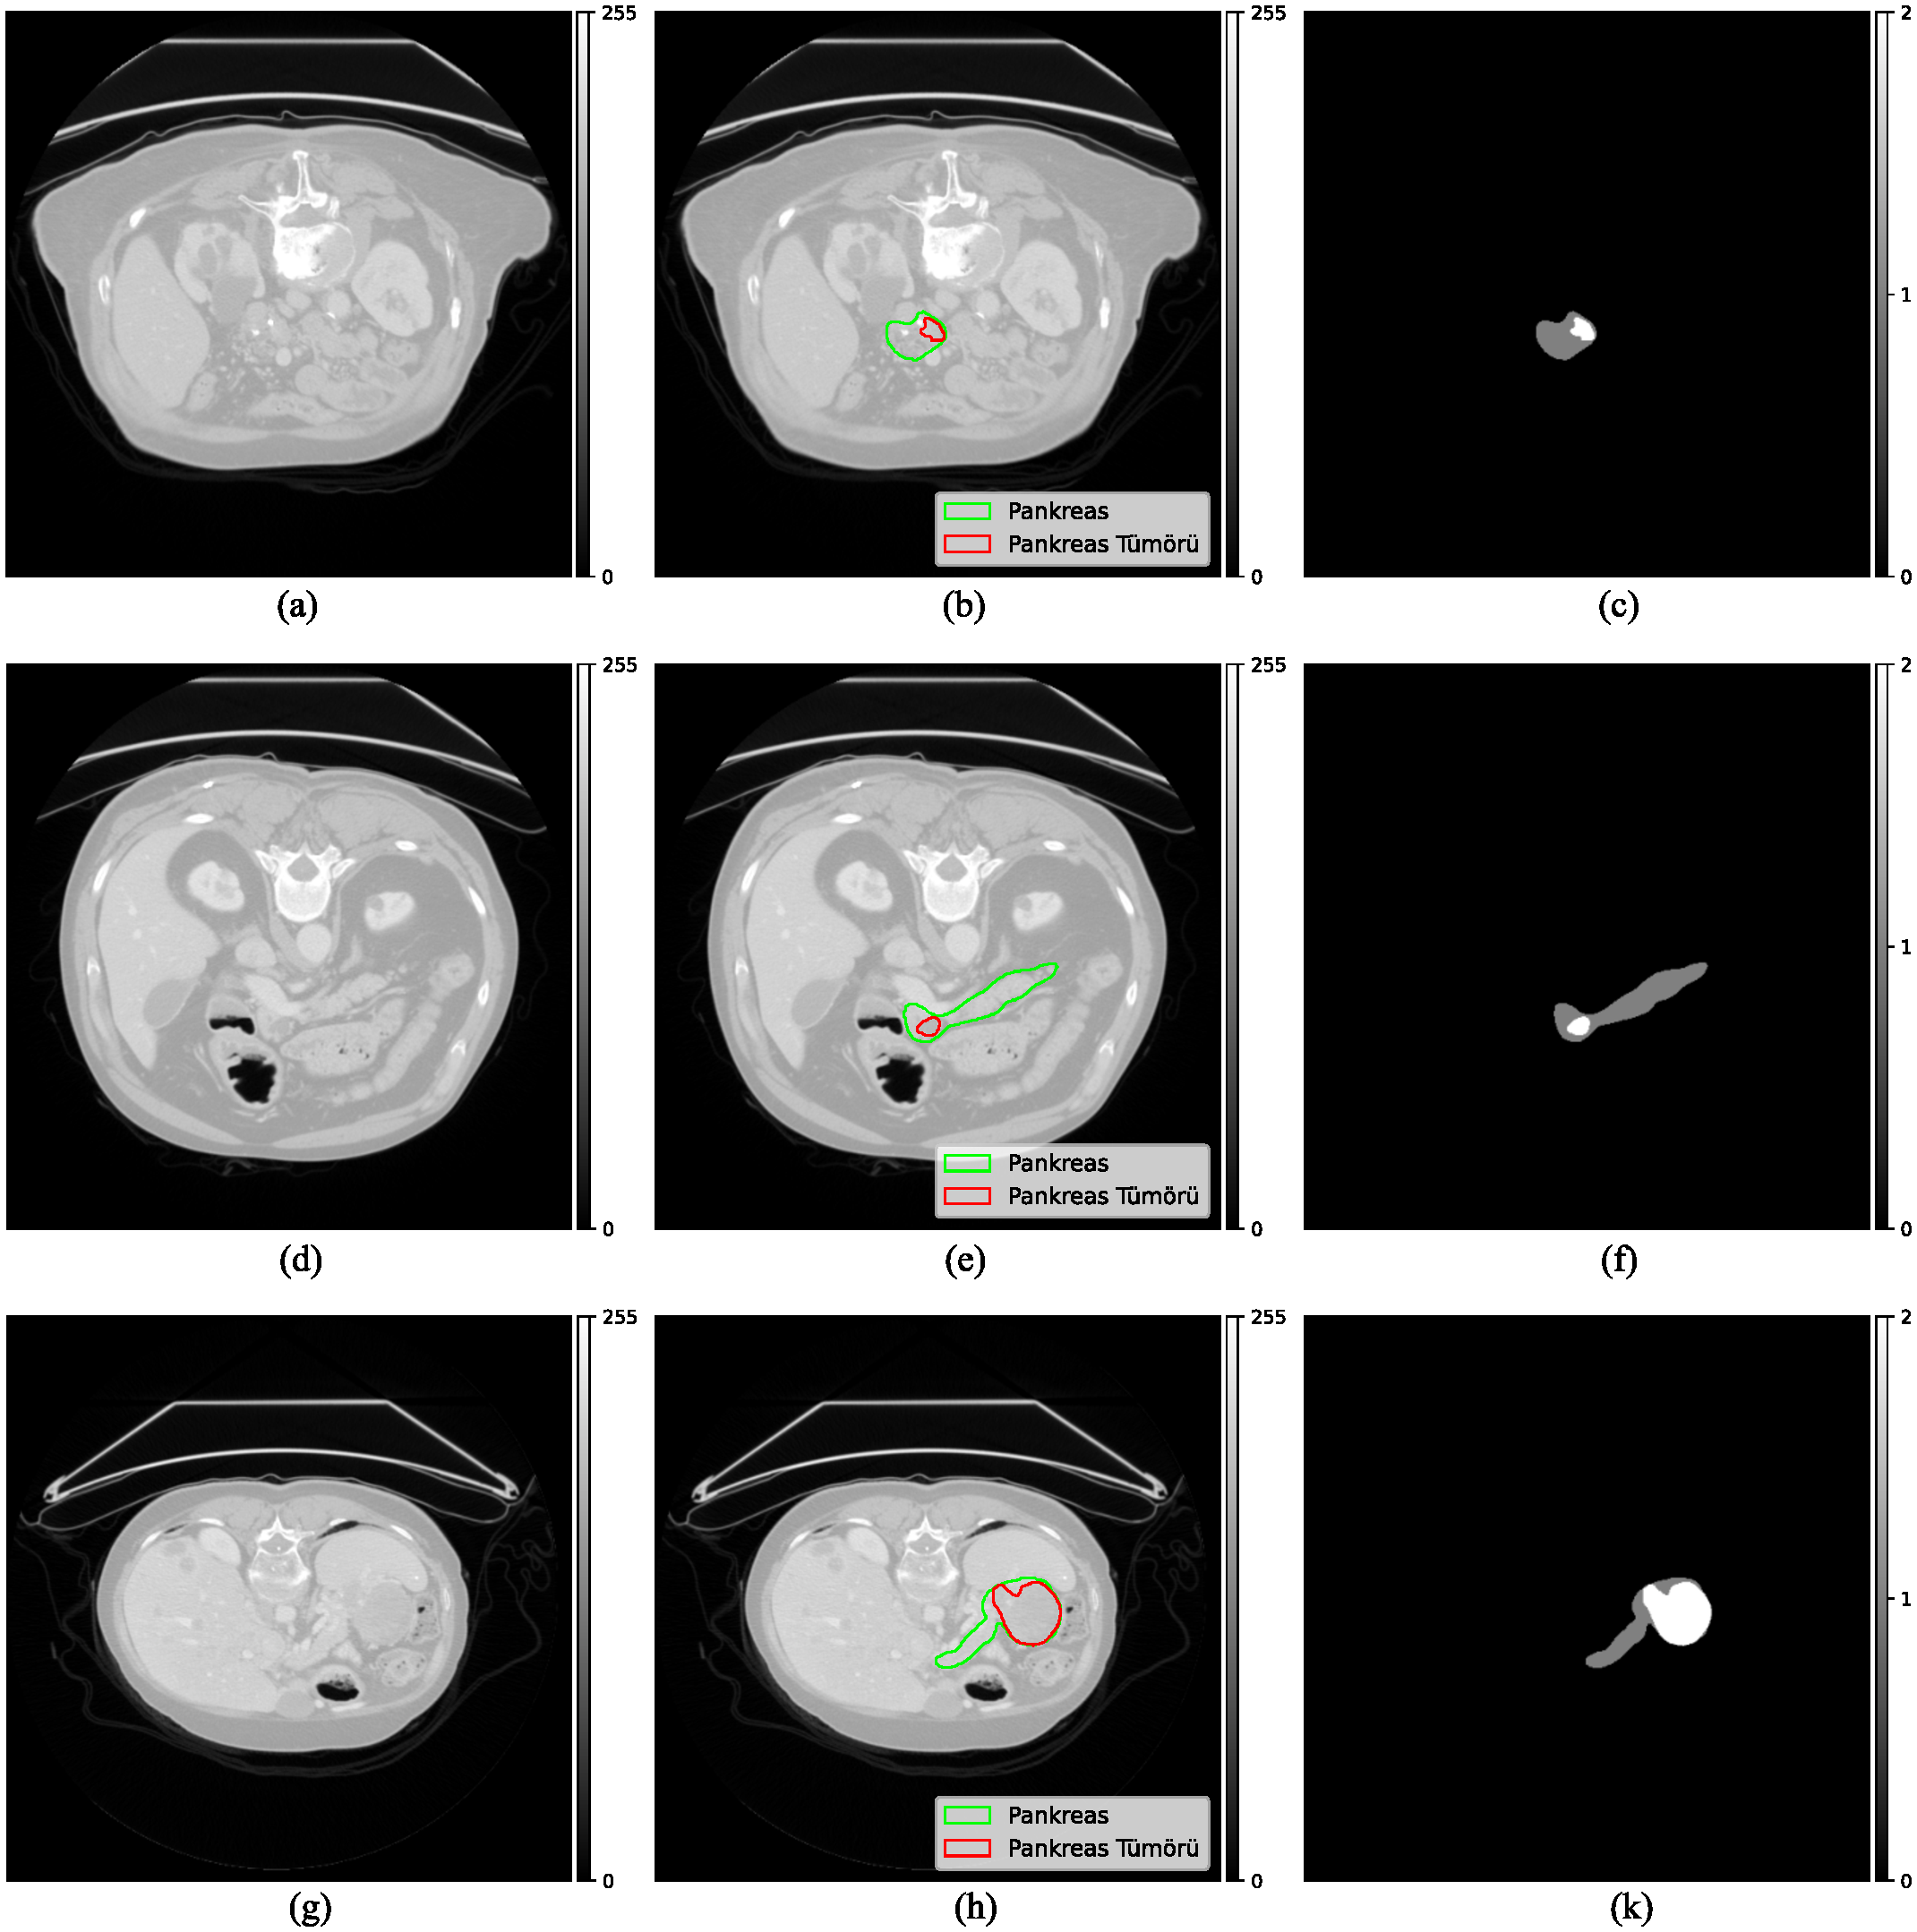
\includegraphics[scale=0.42]{Yapilan-Calismalar/Figures/msd_2dslices.pdf}
		}
	\end{center}
\end{figure} 

Tez çalışmasının ikinci kısmında Pankreas İlgi Bölgesinin Belirlenmesi ve Pankreas ve Pankreas Tümör Segmentasyonu fazlarının test ve eğitimi için Tıbbi Bölümleme Decathlon veri seti \%80 eğitim ve \%20 test olmak üzere iki parçaya ayrılmaktadır. Ayrıca, eğitim seti 4 rastgele gruba ayrılmakta ve 4-kat çapraz doğrulama gerçekleştirilmektedir. Üç set alt eğitim için, bir set ise validasyon için kullanılmaktadır. Alt eğitim ve validasyon seti, derin ağlarda parametre ayarlaması yapmak için kullanılmaktadır. En iyi ağ, sinir ağının eğitimi sırasında gerçekleştirilen validasyon ile elde edilen doğruluk ve hataya bağlı olarak belirlenmektedir. Ardından, çok katmanlı derin ağ mimarilerinin performansı test seti üzerinde ölçülmektedir.

\section{Performans Değerlendirme Metrikleri}
Tez çalışması kapsamında önerilen yaklaşımların değerlendirilmeleri için bilgisayarlı tomografi görüntülerinden oluşan ve farklı özelliklere sahip veri setleri kullanılmaktadır. Önerilen yaklaşımların performans analizleri elde edilen veri tabanları üzerinde gerçekleştirilen deneyler ile irdelenmekte ve literatürde var olan çalışmalara ait sonuçlarla kıyaslamaları gerçekleştirilmektedir. 

Çalışmada kullanılan performans değerlendirme metrikleri şu şekilde açıklanabilmektedir:

\begin{itemize}
	\item Dice Benzerlik Katsayısı (Dice Similarity Coefficient - DSC): Dice benzerlik katsayısı, el ile uzman kişi tarafından işaretlenmiş kesin referans bölgeler ile segment edilen bölgeler arasındaki benzerliği ölçmektedir \cite{dice1945measures}. Bu ölçüt Eşitlik \ref{eq:dsc_metric}’deki gibi hesaplanmaktadır.
	{\setlength{\mathindent}{0cm}
	\begin{equation}    
		\label{eq:dsc_metric}
		DSC=\frac{2 DP}{2 DP+YP+YN}
	\end{equation}}
	Eşitlik \ref{eq:dsc_metric}’de DP, YP ve YN sırasıyla, doğru pozitif, yanlış pozitif ve yanlış negatif sayılarını ifade etmektedir.
	
	\item Jaccard İndeksi (Jaccard Index - JI): Jaccard indeksi, uzman kişi tarafından manuel olarak tespit edilmiş kesin referans bölgelerle yaklaşım tarafından segment edilen bölgeler arasındaki benzerliği ölçmek için kullanılmaktadır \cite{jaccard1912distribution}. Bu değerlendirme prosedürü Eşitlik \ref{eq:ji_metric} kullanılarak temsil edilmektedir. 
	{\setlength{\mathindent}{0cm}
	\begin{equation}
		\label{eq:ji_metric}
		JI=\frac{DP}{DP+YP+YN}
	\end{equation}}
	Eşitlikte DP, YP ve YN sırasıyla, doğru pozitif, yanlış pozitif ve yanlış negatif sayısını temsil etmektedir. 
	
	\item Duyarlılık (Sensivity, Recall - REC): Duyarlılık performans değerlendirme metriği, segmentasyon yaklaşımı tarafından çıkarılan bölgenin piksel sayısının toplam piksel sayısına oranını göstermektedir \cite{altman1994diagnostic}. Bu değerlendirme metriği Eşitlik \ref{eq:rec_metric} kullanılarak elde edilmektedir.
	{\setlength{\mathindent}{0cm}
	\begin{equation}
		\label{eq:rec_metric}
		REC=\frac{DP}{DP+YN}
	\end{equation}}
	Eşitlikte DP ve YN sırasıyla, doğru pozitif ve yanlış negatif değerlerini temsil etmektedir.
	
	\item Özgüllük (Specificity - SPE): Özgüllük performans değerlendirme metriği, arka plan olarak segment edilen bölgenin piksel sayısının bölgenin toplam piksel sayısına oranını bulmak için kullanılmaktadır \cite{altman1994diagnostic}. Bu değerlendirme metriği Eşitlik \ref{eq:spe_metric} kullanılarak elde edilmektedir.
	{\setlength{\mathindent}{0cm}
	\begin{equation}
		\label{eq:spe_metric}
		SPE=\frac{DN}{DN+YP}
	\end{equation}}
	Eşitlikte DN ve YP sırasıyla, doğru negatif ve yanlış pozitif sayısını ifade etmektedir.
	
	\item Kesinlik (Precision - PRE): Kesinlik performans değerlendirme metriği, segmentasyon yaklaşımı tarafından çıkarılan bölgenin gerçekte ne kadar doğru olduğunu göstermekte kullanılmaktadır \cite{altman1994statistics}. Bu değerlendirme metriği Eşitlik \ref{eq:pre_metric} kullanılarak hesaplanmaktadır. 
	{\setlength{\mathindent}{0cm}
	\begin{equation}
		\label{eq:pre_metric}
		PRE=\frac{DP}{DP+YP}
	\end{equation}}
	Eşitlikte DP ve YP sırasıyla, doğru pozitif ve yanlış pozitif değerlerini temsil etmektedir.
	
	\item Doğruluk (Accuracy - ACC): Doğruluk performans değerlendirme metriği, segmentasyon yaklaşımı tarafından çıkarılan bölgenin piksel sayısının toplam piksel sayısına oranını göstermektedir \cite{metz1978basic}. Bu değerlendirme metriği Eşitlik \ref{eq:acc_metric} kullanılarak elde edilmektedir.
	{\setlength{\mathindent}{0cm}
	\begin{equation}
		\label{eq:acc_metric}
		ACC=\frac{DP+DN}{DP+DN+YP+YN}
	\end{equation}}
	Eşitlikte DP, DN, YP ve YN sırasıyla, doğru pozitif, doğru negatif, yanlış pozitif ve yanlış negatif sayısını temsil etmektedir.
	
	Yukarıdaki eşitliklerde DP (Doğru Pozitif) doğru olarak segmentlere ayrılmış bölgeyi, YP (Yanlış Pozitif) yanlış segmentlere ayrılmış bölgeyi ve YN (Yanlış Negatif) eksik olarak segmentlere ayrılmış bölgeyi temsil etmektedir.
	
	\item Alıcı Çalışma Karakteristikleri (Receiver Operating Characteristics - ROC) Eğrisi: ROC eğrisi performans değerlendirme metriği, uzman kişi tarafından manuel olarak tespit edilmiş kesin referans bölgelerle yaklaşım tarafından segment edilen bölgeler arasındaki benzerliği ölçmek için kullanılmaktadır \cite{metz1978basic,fawcett2006introduction}. Segmentasyon yaklaşımının ROC eğrisini çizmek için Spesifiklik (Yanlış Pozitif oranı) ve Duyarlılık (doğru pozitif oranı) olmak üzere iki metrik gerekmektedir.
	
	\item ROC Eğrisinin Alt Alanı (Area under the ROC Curve – AUC): AUC, ROC eğrisinin üzerindeki alanlar ile ROC eğrisinin altındaki alanlar arasındaki farkı ifade etmektedir \cite{hanley1982meaning}. Bu değerlendirme metriği Eşitlik \ref{eq:auc_metric} kullanılarak elde edilmektedir.
	{\setlength{\mathindent}{0cm}
	\begin{equation}
		\label{eq:auc_metric}
		AUC=\int_{x}^{y} f(i) d_{i}
	\end{equation}}
	Eşitlik \ref{eq:auc_metric}'de $f(i)$ ROC eğrisinin üstünde ve altındaki alanları temsil eden bir fonksiyondur. '$x$' ve '$y$', ROC eğrisindeki minimum ve maksimum eksen noktalarını ifade etmektedir.	
\end{itemize}

İdeal pankreas ve pankreas tümör segmentasyonu yaklaşımı ile elde edilen DSC, JI, PRE, REC, ACC, SPE ve AUC değerlerinin diğer yaklaşımlardan daha yüksek olması beklenmektedir.

\section{Literatür Çalışmaları}

Bu tez çalışmasında öncelikle sadece pankreas verilerinin manuel işaretli olduğu NIH veri seti kullanılarak pankreas segmentasyonunun gerçekleştirilmesine yönelik bir yöntem önerilmektedir. Daha sonra pankreas ve pankreas tümör dokularının ayrı ayrı işaretli olduğu MSD veri seti üzerinde farklı derin öğrenme modelleri kullanılarak önerilen yöntemin performansında iyileştirmeler gerçekleştirilmektedir.

Yapılan tez çalışmasının ilk kısmı olan otomatik pankreas segmentasyonu yıllardır aktif olarak çalışılan alanlardan biridir. Bu alan için literatürde birçok çalışma geliştirilmiştir. Bu çalışmalar kronolojik sıraya göre bölge temelli, atlas temelli, model temelli ve derin öğrenme temelli olmak üzere 4 ana grupta ele alınmaktadır. Günümüzde pankreas ve pankreas tümör dokularının segmentasyonuna yönelik çalışmalar derin öğrenme temelli yöntemlerin güçlü segmentasyon sonuçları üretebilmesinden dolayı genellikle derin öğrenme ile gerçekleştirilmektedir.

\subsection{Pankreas Segmentasyonu İçin Kullanılan Bölge Temelli Çalışmalar}

Bölge temelli segmentasyon yaklaşımı en popüler algoritmalardan biridir. Bu çalışmalarda tüm piksellerin anlamlı bölgeleri çıkarılmaktadır. Bölge temelli çalışmalar dört kategoriye ayrılabilmektedirler: 

\begin{enumerate}
    \item Bölge Büyütme Yöntemi: Bu yöntem basitliği ve iyi performansı nedeniyle segmentasyon için en popüler tekniklerden biridir. Çalışma prensibi, bir noktadan başlayarak, komşu piksellerin homojenliği temelinde bir bölge büyütmek, homojen ve bağlantılı bir bölge elde edilene kadar tüm süreci yinelemektir. 2015 yılında Tam ve Nguyen, pankreası BT görüntülerinden segmentlere ayırmak için bölge büyütme ve histogram eşitleme tekniklerini kullanmakta ve Jaccard indeksini 86.87 ile oldukça yüksek sonuçlar elde etmektedirler \cite{tam2014efficient}.

Avantajları: Bağlantılı bölgeler garanti edilmektedir. 

Dezavantajları: Başlangıç noktasını elde etmek için manuel etkileşim gerektirmekte ve aşırı segmentasyona neden olan gürültüye duyarlıdır. 

    \item Böl ve Birleştir Yöntemi: Bu yöntem görüntünün tamamı üzerinde çalışmakta ve homojenliği ayırt etmek için dörtlü ağaç verilerini kullanmaktadır. İşlem süreci, görüntünün tamamının rastgele bağlantısız alt bölgelere bölünmesi ve ardından bu alt bölgelerin makul görüntü bölümlendirme koşulu temelinde birleştirilmesidir. Pankreas segmentasyonu için, bölge ayırma ve birleştirmeye dayalı yöntem tatmin edici segmentasyon sonuçları elde edememektedir \cite{farag2017automatic}. 

    Avantajları: Bağlantılı bölgeler garanti edilmektedir. 

    Dezavantajları: Görüntünün konumu ve yönü, bloklu son segmentasyona yol açmaktadır.
    
    \item Kümeleme Yöntemi: Bu yöntem daha klasik ve yaygın olarak kullanılmaktadır. Temel amacı, aynı özelliklere sahip piksellere benzemektir. K-ortalama kümeleme, nokta değeri ile bu kümenin ortalama değeri arasındaki farkın en küçük olduğu kümeye p noktası ekleyerek tüm görüntüyü k kümeye veya gruba bölmektedir.

    Avantajları: Basit ve kullanışlıdır, genellikle tıbbi görüntüleme ve güvenlik sistemleri için geçerlidir.

    Dezavantajları: K-ortalama kümeleme gibi bazı kümeleme algoritmaları, sürekli bölgeyi garanti edememektedir. 

    \item Eşikleme Yöntemi: Bu yöntem bölütlenecek nesneyi (ön planı) arka plandan ayırmak için görüntünün histogram gibi global bilgilerini kullanmaktadır. 
    
    Avantajları: Basit ve kullanışlıdır.

    Dezavantajları: Eşiği tam olarak belirlemek zordur. 

\end{enumerate}


\subsection{Pankreas Segmentasyonu İçin Kullanılan Atlas Temelli Çalışmalar}
Bu teknikler görüntülerde pankreas varlığı hakkında ön fikir veren bir harita oluşturmaktadır. Araştırmacılar bu çalışmalarda pankreasın bölge ve boyutunu kestirmek için regresyon ormanı yöntemi \cite{oda2016regression}, ağırlıklı alt uzaysal olasılık atlasları \cite{karasawa2015pancreas}, yapıya özel atlas üretimi \cite{karasawa2015pancreas},  pankreas dokusu çevresindeki damar yapısına dayanan atlas seçim stratejisi \cite{karasawa2017multi}, atlas seçimi ve grafik kesime dayalı yöntem \cite{oda2011organ}, mekansal olarak bölünmüş olasılık atlaslarına dayanan otomatik yöntem \cite{chu2013multi}, hiyerarşik atlas kaydı ve ağırlıklandırma şemasına dayanan yöntem \cite{wolz2013automated}, segmentasyon doğruluğuna ve etkileşim maliyetlerine dayalı yöntem \cite{takizawa2017interactive}, hastaya özel olasılık atlas rehberli segmentasyon yöntemi \cite{shimizu2010automated}, koşullu şekil -- konum ve denetimsiz yoğunluk öncelikleri temelli yöntem \cite{okada2015abdominal} geliştirmişlerdir. Bu tekniklerin en kritik dezavantajlarından biri hesaplama maliyetinin oldukça yüksek olmasıdır.

\subsection{Pankreas Segmentasyonu İçin Kullanılan Model Temelli Çalışmalar}
Bu teknikler pankreasın segmentasyonu için pankreas istatistiksel şekil modelini uyarlamaktadırlar \cite{hammon2013model}.  Pankreasın farklı anatomik yapısı nedeniyle, bu teknikler tatmin edici sonuçlar verememektedirler.

\subsection{Pankreas Segmentasyonu İçin Kullanılan Derin Öğrenme Temelli Çalışmalar}
Derin Sinir Ağları (Deep Neural Network - DNN) tabanlı tekniklerde pankreastaki etkin özellikler doğrudan görüntü verilerinden elde edilmektedir. Derin sinir ağlarının hızla gelişmesi ile sınıflandırma \cite{roth2015deep,roth2015deeporgan}, lokalizasyon \cite{roth2016spatial,roth2018spatial}, tanıma \cite{zhou2016pancreas,cai2017improving}, segmentasyon \cite{yu2018recurrent,ma2018novel,zhu20183d} ve hizalama \cite{roth2015deeporgan,chen2019harnessing} gibi birçok tıbbi görüntü işleme ve bilgisayarla görme uygulamalarında tatmin edici performanslar elde edilmektedir. Bunun üzerine araştırmacılar derin öğrenme (DÖ) yöntemlerini kullanarak pankreas segmentasyonu için daha yüksek doğruluklu sonuçlar elde etmeye başlamışlardır. Otomatik pankreas segmentasyonu için DÖ yöntemlerini kullanan literatür çalışmaları pankreas segmentasyonu başarısını önemli ölçüde artırmıştır. Son yıllarda pankreas segmentasyon başarısının artması ile derin öğrenme temelli yaklaşımlar pankreas tümör segmentasyonunda da kullanılmaya başlanmıştır. Bu amaçla 3 sınıflı (Pankreas, Pankreas Tümörü, Diğer dokular) MSD gibi veri setleri araştırmacıların açık erişimine açılmıştır.

\subsubsection{Sadece Pankreas Organının Segmentasyonuna Yönelik Gerçekleştirilen Derin Öğrenme Temelli Akademik Çalışmalar}
Bu tez çalışmasında pankreas segmentasyonu için iki aşamalı derin öğrenme esaslı bir yöntem önerilmiştir. Bu çalışmada kullanılan derin öğrenme tekniklerini kullanarak pankreas segmentasyonu gerçekleştiren benzer çalışmalar ve bu çalışmaların başarıları Tablo \ref{tab:lit1}'deki gibi özetlenebilmektedir.

\begin{table}[h!]
	\centering
	\caption{Otomatik pankreas segmentasyonu için derin öğrenme yöntemlerini kullanan literatür çalışmaları}
	\label{tab:lit1}
	\begin{tabular}{cccccc}
		\toprule
		Metot                           &  Veri Seti   &  Model              & Başarı (DSC\%)  \\ 
		\midrule 
		Roth 2015 - 1 \cite{roth2015deep}  &  NIH-82    &  Hierarchical Coarse-to-Fine          & 68$\pm$10   \\ 
		Roth 2015 - 2 \cite{roth2015deeporgan}  &  NIH-82    &  ConvNets                             & 71,8$\pm$10,7 \\
		Roth 2016     \cite{roth2016spatial}    &  NIH-82    &  Holistically Nested Network          & 78,01$\pm$8,2 \\
		Roth 2018     \cite{roth2018spatial}    &  NIH-82    &  Holistically Nested Network          & 81,27$\pm$6,27\\
		Zhou 2016     \cite{zhou2016pancreas}    &  NIH-82    &  Coarse-to-Fine                       & 82,37$\pm$5,68\\
		Cai 2017      \cite{cai2017improving}     &  NIH-82    &  Recurrent Neural Contextual Learning & 82,4$\pm$6,7 \\
		Yu  2017      \cite{yu2018recurrent}      &  NIH-82    &  Saliency Transformation Network      & 84,5$\pm$4,97 \\
		Ma 2018       \cite{ma2018novel}      &  NIH-82    &  Bayesian Model                      & 85,32$\pm$4,19 \\
		Zhu 2018      \cite{zhu20183d}     &  NIH-82    &  3D Coarse-to-Fine                   & 84,59$\pm$4,86 \\
		Zhao 2019     \cite{zhao2019fully}    &  NIH-82    &  3D U-Net                             & 85,99$\pm$4,51 \\
		Chen 2019     \cite{chen2019harnessing}    &  NIH-82    &  3D Coarse-to-Fine                   & 85,22$\pm$4,07 \\
		Khosravan 2019\cite{khosravan2019pan}& NIH-82    &  Projective Adversial Network        & 85,53$\pm$1,23 \\
		Li 2019       \cite{li2020model}       &  NIH-82    &  Model Driven Stack - based FCN      & 83,5$\pm$6,2  \\
		Xue 2019       \cite{xue2019cascaded}     &  NIH-82    &  Cascaded 3D FCN      & 85,9$\pm$5,1  \\	
		Liu 2019       \cite{liu2019automatic}     &  NIH-82    &  Ensemble-based FCN  & 84,10$\pm$4,91  \\		 
		Zheng 2020     \cite{zheng2020deep}  &  NIH-82    &  2D U-Net      & 84,37 \\	 
		Zhou 2017    \cite{zhou2017deep}     &  JHMI      &  Deep Supervision  & 79,23$\pm$27,71   \\
		Zhu 2018      \cite{zhu20183d}      &  JHMI      &  3D Coarse-to-Fine & 80,56$\pm$13,36   \\
		\bottomrule
	\end{tabular}
\end{table}

Pankreas segmentasyonu için popüler derin öğrenme ağ modellerinde sıklıkla kullanılan konvolüsyon katmanlarını kullanan ilk çalışma Roth tarafından geliştirilmiştir \cite{roth2015deep}. Bu çalışmada NIH pankreas veri seti oluşturulmuş ve yerel görüntü bölgeleri (pankreas) Hiyerarşik Kabadan İnce (Hierarchical Coarse-to-Fine) modele dayanan bir yöntem kullanılarak sınıflandırılmıştır. Daha sonra Roth, 2B görüntü dizilerindeki pikselleri piksel başına maskeleme aracılığıyla bağımsız olarak işleyen Holistik İç İçe Evrişimsel Sinir Ağları (Holistically-Nested Convolutional Neural Networks) ile pankreas segmentasyon performansını geliştirmiştir \cite{roth2016spatial,roth2018spatial}. Zhou, Kabadan İnceye (Coarse-to-Fine) yaklaşımıyla pankreas segmentasyonu gerçekleştiren bir çalışma geliştirmiştir \cite{zhou2016pancreas}. Bu yaklaşımda öncelikle kaba ölçekli faz ile kaba olarak pankreas bölgesi çıkarılmaktadır. Daha sonra ince ölçekli fazda bu kaba bölgeler tekrar sınıflandırılarak detaylı pankreas bölgesi elde edilmektedir. Performans bakımından yeterli olsa da, kaba ve ince ölçekli fazların ayrı ayrı eğitimi ve test edilmesi nedeniyle daha yüksek hesaplama maliyeti gibi bazı dezavantajları mevcuttur. Bağlamsal öğrenme ve segmentasyonun tutarlılık sorununu çözmek için Cai, Bağlamsal Tekrarlayan Sinir Ağları (Contextual Recurrent Neural Networks: CRNN) yaklaşımını önermiştir \cite{cai2017improving}. Yu, kaba ve ince ölçekli fazları Belirgin Dönüşüm Ağı (Saliency Transformation Network) aracılığıyla birbirine bağlayarak Zhou tarafından önerilen \cite{zhou2016pancreas} önceki yaklaşımın performansını geliştirmiştir \cite{yu2018recurrent}. Ma, derin sinir ağı ve istatistiksel şekil modelinin segmentasyon sonuçlarının birleştirildiği Bayes modeline dayanan hibrit bir yaklaşım önermiştir \cite{ma2018novel}. 

Literatür çalışmalarında, 2B CNN’ye dayalı tekniklerin BT’nin üçüncü boyuttaki bilgilerinin elde edilmesinde kısıtlamalara sahip olduğu bildirilmektedir. Bu nedenle, 2B ağlara göre önemli ölçüde daha yüksek hesaplama gücü ve bellek gerektiren 3B ağlar kullanılarak (3B U-Net \cite{zhao2019fully}, 3B Kabadan İnceye (3D Coarse-to-Fine) \cite{zhu20183d,chen2019harnessing}, 3B Tamamen Konvolüsyonel Ağlar (Fully Convolutional Networks : FCN) \cite{roth2018application}, Projektif Çekişmeli Ağlar (Projective Adversarial Networks : PAN) \cite{khosravan2019pan}, Kaskat 3B FCN (Cascaded 3D FCN) \cite{xue2019cascaded}) daha yüksek başarıya sahip pankreas segmentasyon sonuçları elde edilmiştir. 

Pankreas segmentasyonu ile ilgili literatür çalışmalarını test etmek için kullanılan bir başka veri seti JHMI patolojik kist veri setidir \cite{zhu20183d,zhou2017deep}. Fakat bu veri seti ilgili araştırmacılar tarafından serbest kullanım için henüz paylaşılmamıştır. Tablo \ref{tab:lit1}’de gösterilen literatür çalışmalarının başarılarına göre, NIH ve JHMI veri setleri için maksimum Dice Benzerlik Katsayısı (Dice Similarity Coefficient - DSC) değerleri 3B U-Net \cite{roth2015deep, farag2016bottom} ve 3B Kabadan İnceye (3D Coarse-to-Fine) \cite{zhu20183d}'de elde edilen \%85.99 ve \%80.56 değerleridir. Bu çalışmalar önceki çalışmalara göre \%17.99 ve \%1.33 iyileştirme sağlamışlardır.

\subsubsection{Pankreas ve Pankreas Tümörü Segmentasyonu İçin Gerçekleştirilen Derin Öğrenme Temelli Akademik Çalışmalar}

Tez çalışmasının ikinci kısmı otomatik pankreas ve pankreas tümör segmentasyonudur. Pankreas ve pankreas tümörünün değişken büyüklüğü, şekli ve konumu nedeniyle literatürde bu alanla ilgili çok çalışma bulunmamaktadır. Yapılan çalışmalar da belirli bir başarı yüzdesine kadar ulaşabilmektedirler. Otomatik pankreas ve pankreas tümörü segmentasyonu için DÖ yöntemlerini kullanan literatür çalışmaları Tablo \ref{tab:lit2}’te listelenmektedir. Bu çalışmalar şu şekilde özetlenebilmektedir: 

\begin{table}[h!]
	\centering
	\caption{Otomatik pankreas ve pankreas tümör segmentasyonu için derin öğrenme yöntemlerini kullanan literatür çalışmaları}
	\label{tab:lit2}
	\begin{adjustbox}{width=\textwidth}
	\begin{tabular}{ccm{5cm}cccc}
		\toprule
		Metot                           &  Veri Seti   &  Model  & Pankreas (DSC\%)  & Tümör (DSC\%) \\ 
		\midrule 
		Isense 2018 \cite{isensee2018nnu}  &  MSD    &  nnU-Net (no-new-Net)  & 79,53 & 52,27  \\ 
		Cai 2019 \cite{cai2019end}  &  MSD   &  Adversarial Shape Learning & 74,3$\pm$12,2 & - \\
		Xia 2020 \cite{xia2020uncertainty}    &  MSD    &  Uncertainty-awere Multi-view Co-training (UMCT)   & 74,93 & - \\
		Yu 2020 \cite{yu2020c2fnas}    &  MSD    & Corse-to-Fine Neural Architecture Search (C2FNAS)   & 80,76 & 54,41\\
		Yu 2021 \cite{yu2020cakes}    &  MSD    & Channel-wise Automatic Kernel Shirinking (CAKES) & 80,12 & 48,72\\
		Zhu 2019 \cite{zhu2019v}     &  MSD    &  V-NAS & 79,94$\pm$8,85 & 37,78$\pm$32,12 \\
		Tureckova 2020 \cite{tureckova2020improving}      &  MSD    &  Deep Supervision and Atentional Gates      & 81,81$\pm$0,98 & 52,68$\pm$1,89 \\
		Xia 2020       \cite{xia20203d}      &  MSD    &  3D Semi Supervised Learning                      & 78,42 & 38,48 \\
		\bottomrule
	\end{tabular}
	\end{adjustbox}
\end{table}

2015 yılında sunulan U-Net, sade ve başarılı yapısı ile tıbbi görüntü segmentasyonunda hızla yaygın olarak kullanılan bir mimari haline gelmiştir. Bununla birlikte, U-Net'in yeni problemlere uyarlanması, kesin mimari, ön işleme, eğitim ve çıkarımla ilgili birkaç serbestlik derecesini içermektedir. Bu seçenekler birbirinden bağımsız olmayıp genel performansı önemli ölçüde etkilemektedir. Isensee çalışmasında U-Net’in bu eksikliklerini minimize etmek amacıyla nnU-Net (no-new-Net)’i önermiştir \cite{isensee2018nnu}. Bu modelde 2B ve 3B U-Net modellerinin temel yapıları birleştirilmektedir. Önerilen bu model, pankreas ve pankreas tümör BT dilimlerini içeren Decathlon veri seti kullanılarak değerlendirilmiştir. 

Karın (abdomel) organlarının genelde şekil ve topolojilerinin farklı olmasından dolayı geleneksel CNN tabanlı segmentasyon modellerini eğitmek zor olmaktadır. Cai çalışmasında bu dezavantajı minimize etmek için Uçtan Uca ve Şekil öğrenme (Adversarial Shape Learning) mimarili yeni bir model önermiştir \cite{cai2019end}. Model girdi olarak derin öğrenme özelliklerini almakta ve organ yüzeyinde bulunan noktalar olarak organ şekli temsillerini üretmektedir. Ek olarak bu çalışmada şekil bilgilerini daha iyi yakalamak ve nokta ağını optimize etmek için yeni bir çekişmeli şekil öğrenme amaç fonksiyonu sunulmaktadır.

Segmentasyon uygulamalarında performansı en üst düzeye çıkarmak için değişen model topolojileri, optimizasyon parametreleri, ön işleme adımları ve model topolojileri geliştirmek standart uygulamalardandır. Fakat bu standart uygulamaların farklı görevlere nasıl aktarıldığı genellikle net değildir. Bu durumu ortadan kaldırmak amacıyla, Perslev çalışmasında tıbbi görüntülerin segmentasyonu için basit ve kapsamlı derin öğrenme modeli önermiştir \cite{perslev2019one}. 

Tıbbi görüntü segmentasyonunda büyük başarı elde etmiş olsa da, derin öğrenmeye dayalı yaklaşımlar genellikle tıbbi görüntü analizi alanında son derece pahalı olabilen, büyük miktarda ve iyi açıklamalı veri gerektirmektedir. Öte yandan, etiketlenmemiş verilerin elde edilmesi çok daha kolaydır. Yarı denetimli öğrenme ve denetimsiz alan uyarlaması, birbirleriyle yakından ilişkili olup etiketlenmemiş verilerden yararlanmaktadır. Xia çalışmasında tıbbi görüntü segmentasyonu (pankreas segmentasyonu) için bu iki görevi ele alan ve birleşik çerçeve olan Belirsizliğe Duyarlı Çoklu Görüş Ortak Eğitimi (Uncertainty-aware Multi-view Co-training  - UMCT) önermiştir \cite{xia2020uncertainty}. Önerilen yöntem daha iyi performans için etiketlenmemiş verileri verimli bir şekilde kullanma yeteneğine sahiptir.

Literatürde 3B konvolüsyonel sinir ağlarının 3B tıbbi görüntülerde organları veya tümörleri ayrıştırmada çok başarılı olduğu kanıtlanmıştır. Ancak farklı görev bağlamları verilen uygun 3B ağları seçmek veya tasarlamak karmaşık ve zaman alıcı olmaya devam etmektedir. Son zamanlarda, en iyi ağ mimarisini otomatik olarak arayarak bu sorunu çözmek için Yapay Mimari Arama (Neural Architecture Search - NAS) algoritmaları önerilmektedir. Yu çalışmasında, ağ boyutu veya giriş boyutunda tutarsızlık olmadan 3B segmentasyon ağını sıfırdan otomatik olarak aramak için Kabadan İnceye Sinir Mimari Araması (Coarse-to-Fine Neural Architecture Search - C2FNAS) önermiştir \cite{yu2020c2fnas}.

3B CNN video analizi ve hacimsel görüntü tanıma gibi 3B sahne anlamada yaygın olarak uygulanmaktadır. Fakat, 3B ağlar pahalı hesaplama maliyetine neden olan aşırı parametrelendirmeye kolayca yol açabilmektedirler. Yu çalışmasında, standart 3B konvolüsyonları bir dizi operasyonla küçülterek verimli 3B öğrenmeyi mümkün kılmak için Kanal Otomatik Çekirdek Küçültmesini (Channel wise Automatic KErnel Shrinking - CAKES) önermiştir \cite{yu2020cakes}.

Derin Öğrenme sistemlerinin güvenilirliği doğruluklarına değil, aynı zamanda girdi verilerindeki olumsuz bozulmalara karşı sağlamlıklarına da bağlıdır. Daza çalışmasında doğal görüntü alanındaki olumsuz gürültü varlığında Derin Sinir Ağlarının performansını iyileştirmek için çeşitli saldırılar ve savunmalar önermiştir \cite{daza2021towards}. Bununla birlikte, bu çalışmada hacimsel veriler için bilgisayar destekli tanılamadaki sağlamlık, yalnızca belirli görevler için ve sınırlı saldırılarla araştırılmıştır.

Derin öğrenme algoritmaları, özellikle 2B ve 3B FCN'ler, hacimsel tıbbi görüntü segmentasyonu için hızla ana metodoloji haline gelmiştir. Fakat, 2B modeller üçüncü eksen boyunca zengin uzamsal bilgiden tam olarak yararlanamazken, 3B modeller zorlu hesaplama ve yüksek GPU bellek tüketiminden muzdariptir. Zhu çalışmasında hacimsel tıbbi görüntü segmentasyonu problemine göre ağ mimarisini otomatik olarak aramayı önermiştir \cite{zhu2019v}. Somut olarak, yapı öğrenimini türevlenebilir sinir mimarisi araştırması olarak formüle etmektedirler. 

BT görüntülerindeki organların segmentasyonu, hasta teşhisi için doktorlara ve radyologlara önemli bir katkı sağlamaktadır. Bir vücut bölgesinin BT taramaları genellikle farklı komşu iç vücut organlarını içermektedir. Derin öğrenme gibi tekniklerle başarılı bir segmentasyon gerçekleştirmek için ağın ilgilenilen organa ve çevreleyen yapılara odaklanmayı öğrenmesi gerekmektedir. Ayrıca ağın farklı büyüklükteki hedef bölgeleri tespit edebilmesi büyük önem taşımaktadır. Tureckova çalışmasında popüler bir derin öğrenme metodolojisi olan Konvolüsyonel Sinir Ağlarına derin denetim ve dikkat kapılarını dahil ederek genişletilmesini sağlamıştır \cite{tureckova2020improving}.

Derin sinir ağları, çeşitli alanlarda önemli bir etki yaratırken, eğitim için genellikle, özellikle tıbbi alanda, birçok uygulamada toplanması pahalı olan büyük miktarda etiketlenmiş veri gerektirmektedir.  Etiketlenmemiş veriler ise çok daha fazladır. Ortak eğitim gibi yarı denetimli öğrenme teknikleri, etiketlenmemiş verilerden yararlanmak için güçlü bir araç sağlayabilmektedirler. Xia çalışmasında, tıbbi görüntülemeden elde edilen hacimsel veriler gibi 3B veriler üzerinde yarı denetimli öğrenmeyi ele almak için Belirsizliğe Duyarlı Çok Görüşlü Ortak Eğitim (Uncertainty-aware Multi-view Co-training - UMCT) adlı yeni bir model önermiştir \cite{xia20203d}. Çalışmada, 3B verilerin çoklu bakış açısı tutarlılığından yararlanılarak ortak eğitim sağlanmaktadır. 

\section{Tezin Kapsamı ve Katkıları}

\subsection{Tezin Kapsamı}

Pankreas organı kalp, beyin, karaciğer veya böbrekler gibi diğer organlarla karşılaştırıldığında daha karmaşık bir anatomik yapıya sahiptir. Yaş, cinsiyet, vücuttaki yağlanma gibi kişisel özellikler pankreasın boyutunu, şeklini ve konumunu etkilemektedir. Pankreas kanseri ise dünya çapında en düşük beş yıllık sağ kalım oranına sahip bir hastalıktır. Pankreas vücudumuzdaki konumu nedeniyle gizli organ olarak adlandırılmaktadır. Pankreas tümörleri gizli konumu nedeniyle genellikle karın üzerinden elle tespit edilememektedir. Pankreas kanserli hastaların çoğu, hastalık ileri bir aşamaya ulaşana kadar asemptomatik kalmaktadır. Pankreas kanseri semptomları genellikle tümör mide, oniki parmak bağırsağı, karaciğer veya safra kesesi gibi diğer yakın organların işlevine müdahale etmeye başlayana kadar ortaya çıkmamaktadır. Bu durum pankreas kanserinin geç tanısına neden olmaktadır \cite{kamisawa2016pancreatic,mizrahi2020pancreatic}. 

\captionsetup[figure]{margin={0.5cm,0cm}}
\begin{figure}[h!]
	\begin{center}
		\vspace{0.4cm}
		\captionbox{Farklı boyut, şekil ve pozisyonda (anatomik yapılar) 2B dilim (a, b, c) ve 3B pankreas modelleri (d, e, f) örnekleri. Pankreasın manuel olarak uzman tarafından işaretlenmiş gerçek referans bölgeleri yeşil renkte gösterilmektedir.
			\label{fig:pancreas_types}}
		{
			\vspace{0.4cm}
			\begin{tabular}{ccc}
				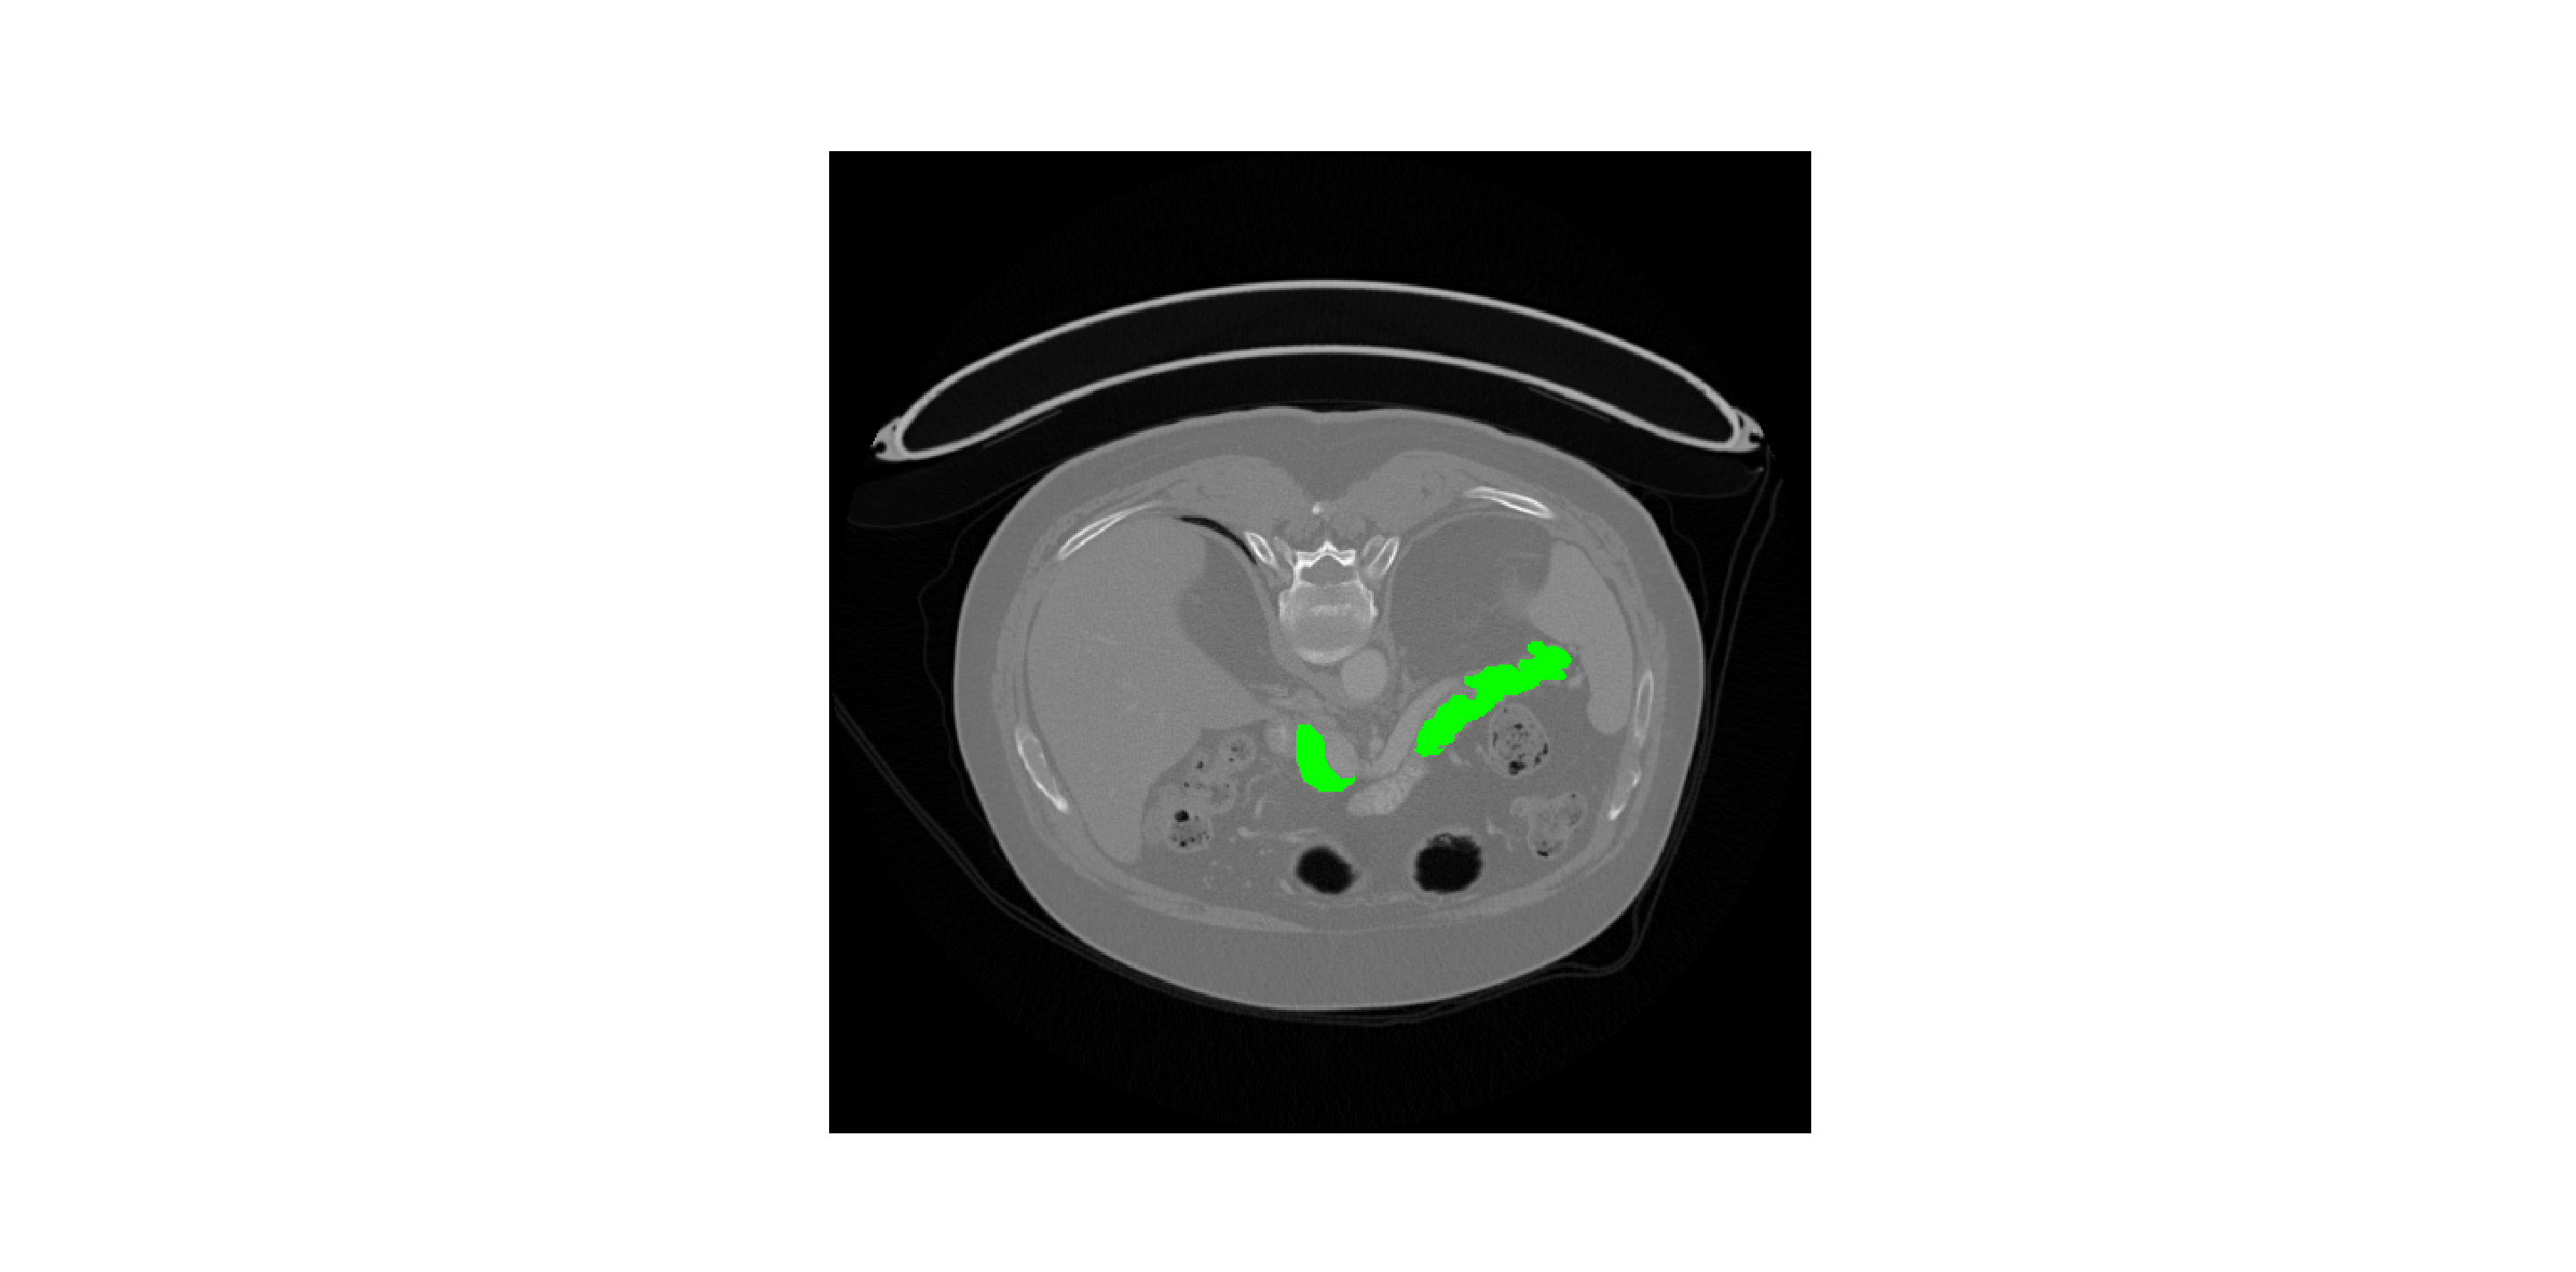
\includegraphics[scale=0.25]{Genel-Bilgiler/Figures/68gt2D.pdf} & 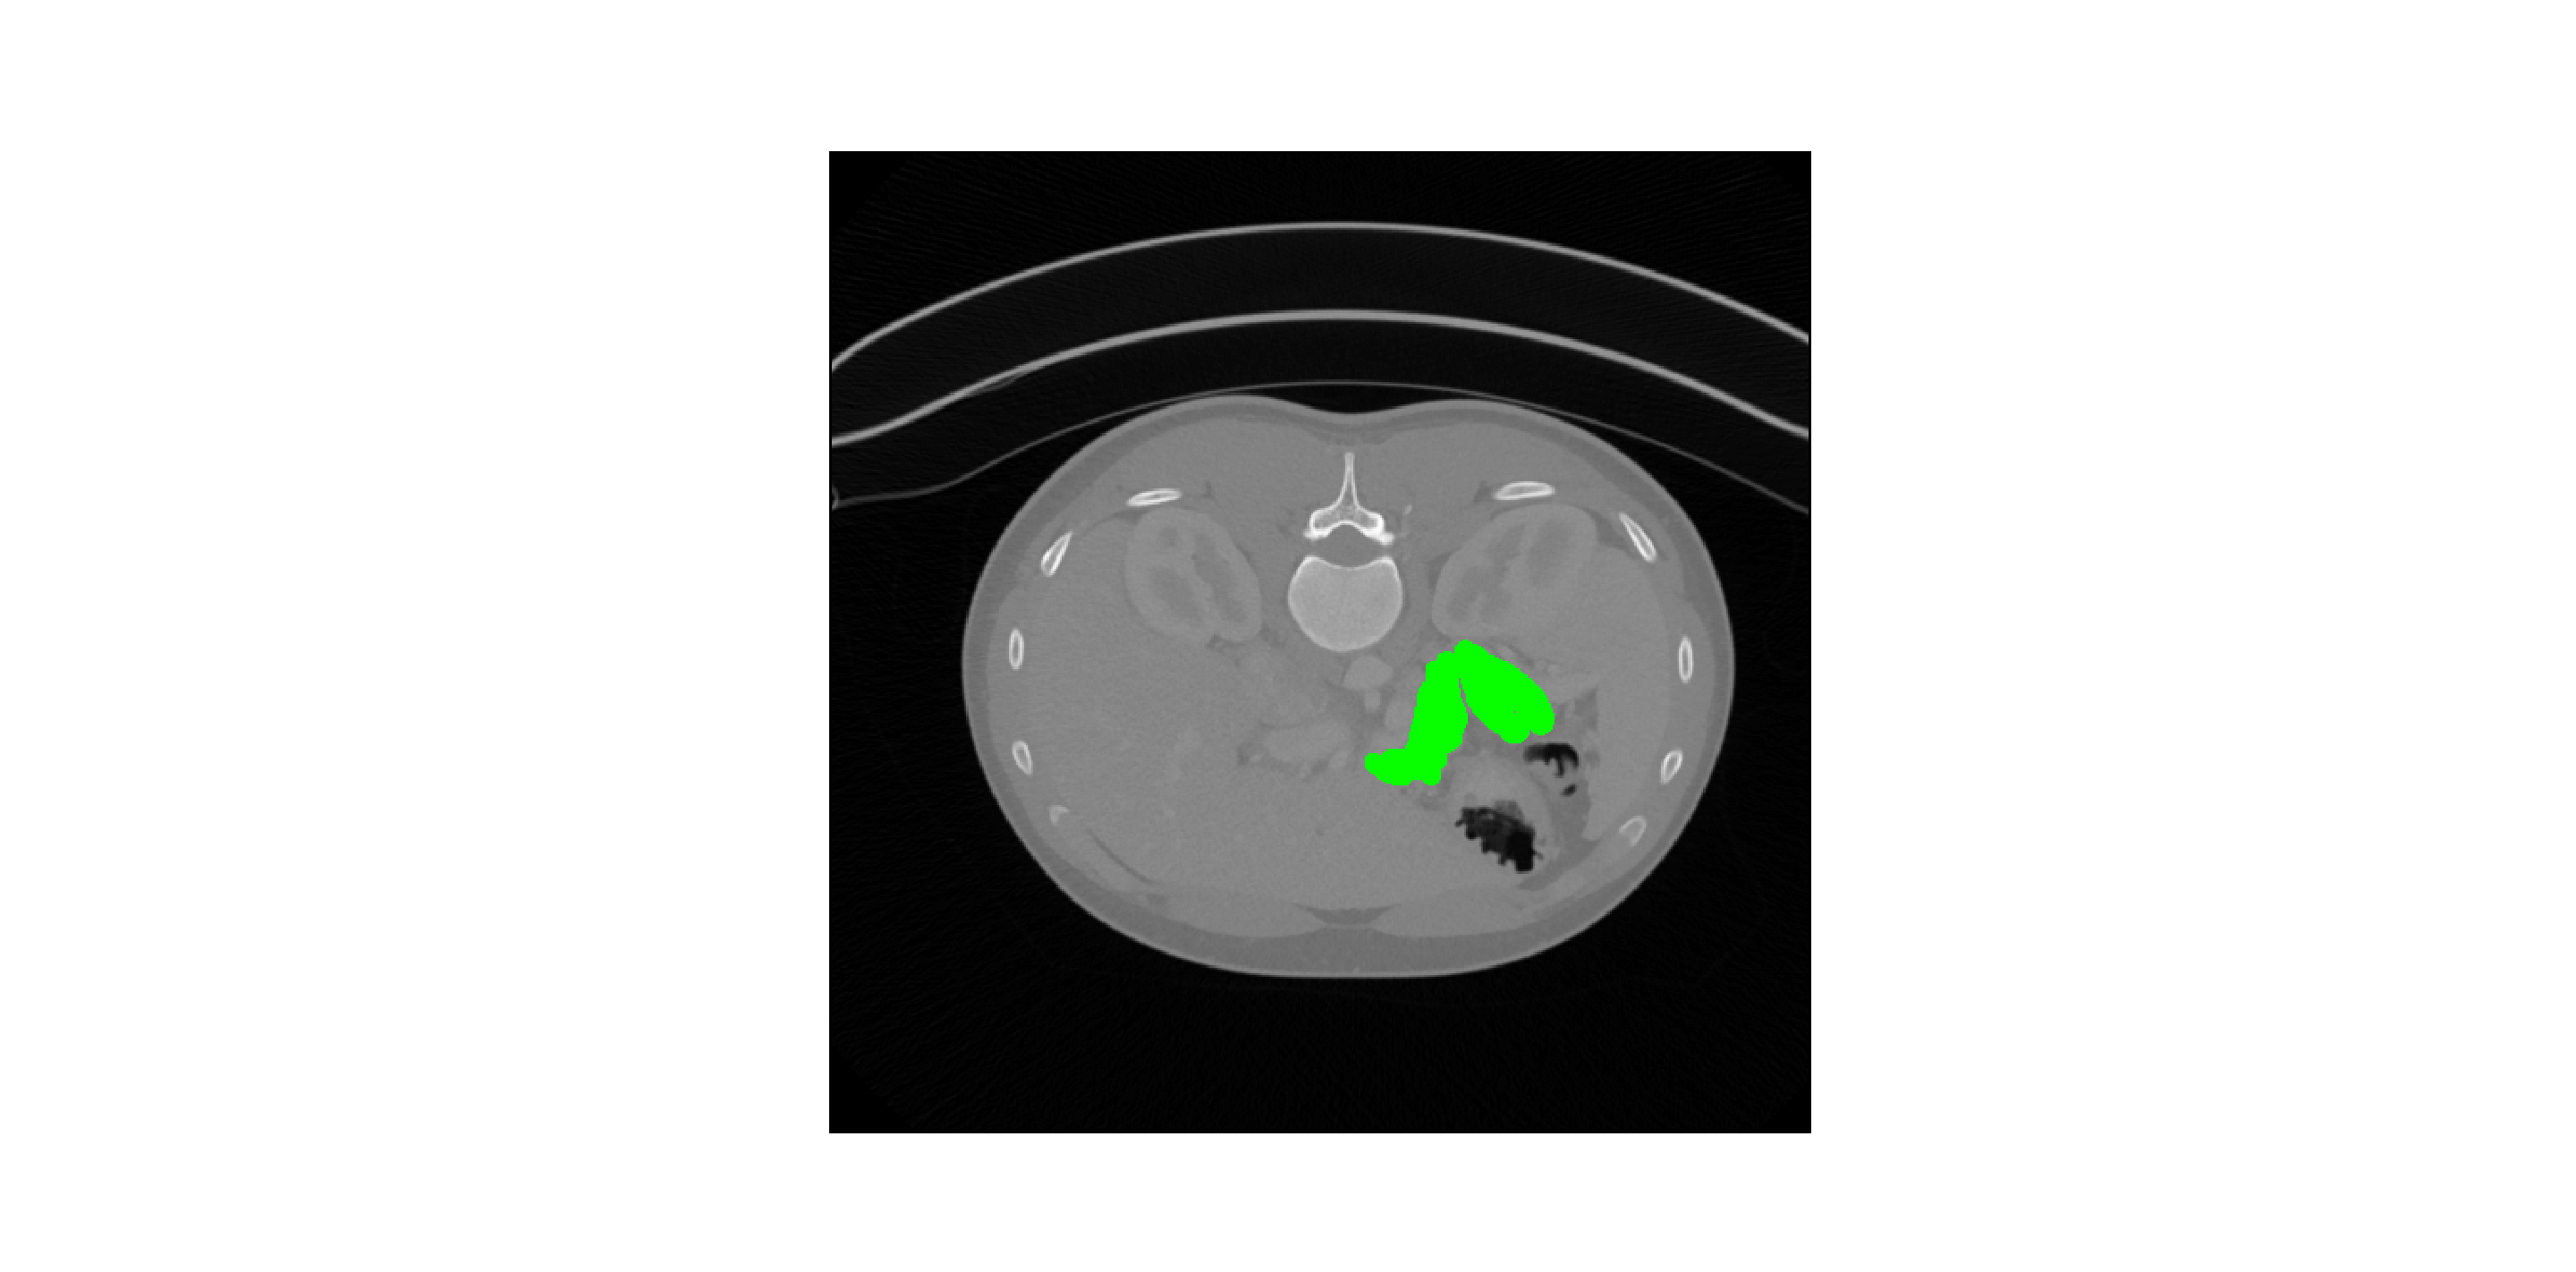
\includegraphics[scale=0.25]{Genel-Bilgiler/Figures/70gt2D.pdf} & 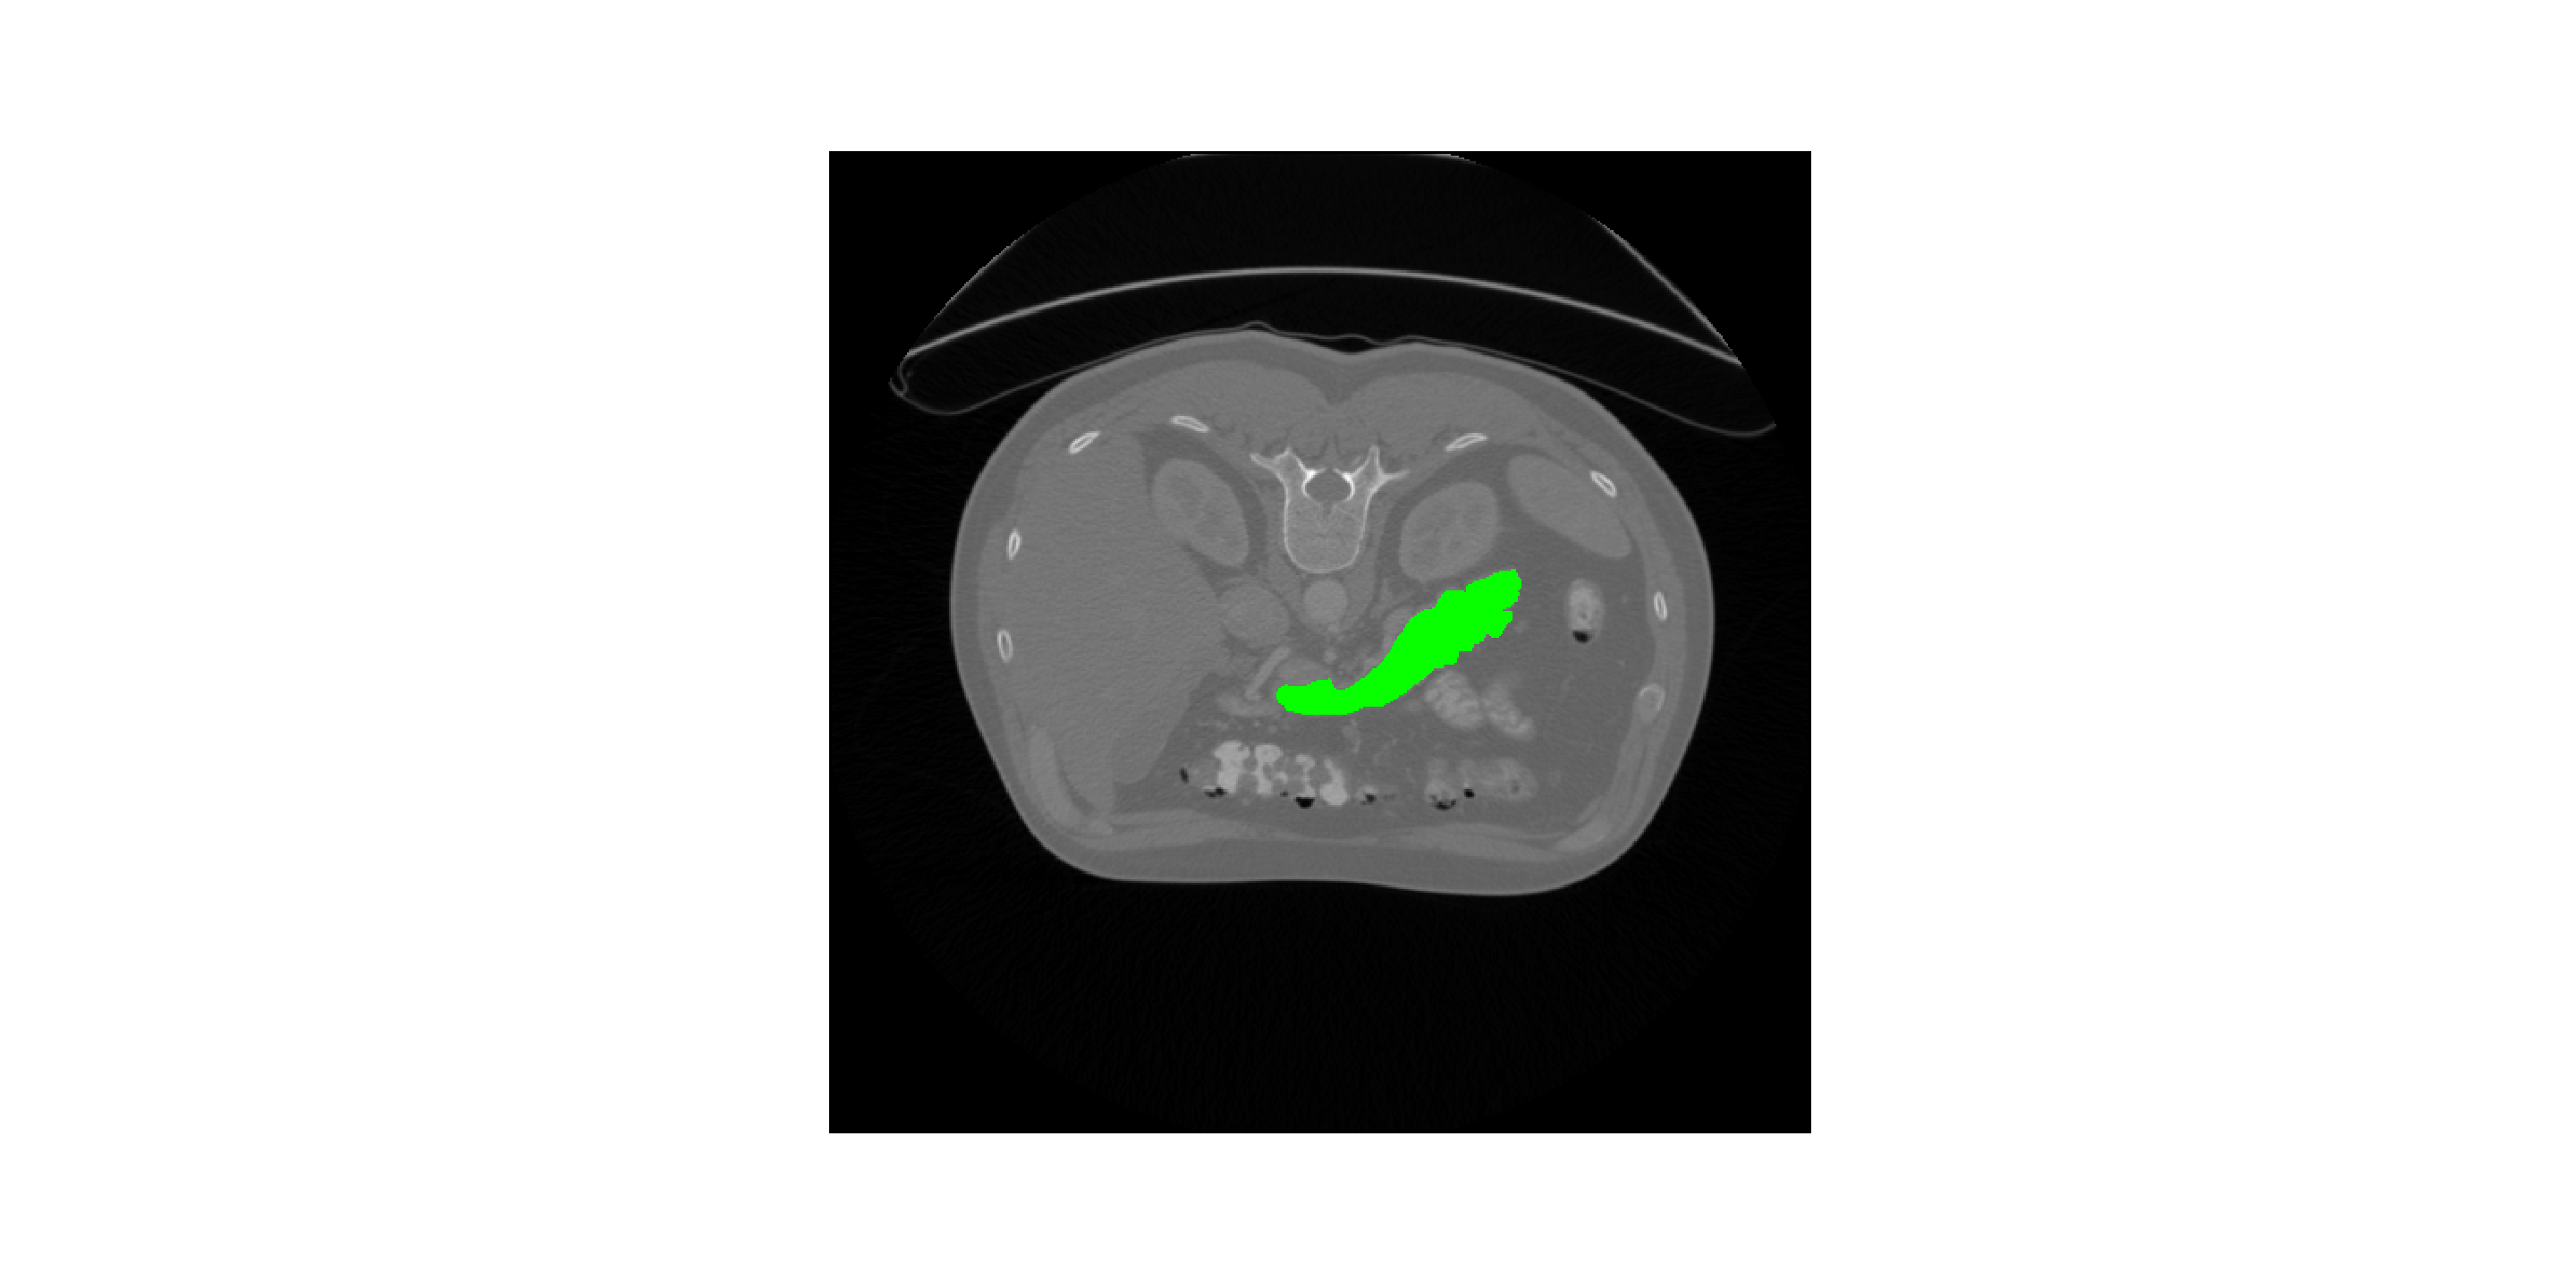
\includegraphics[scale=0.25]{Genel-Bilgiler/Figures/74gt2D.pdf} \\
				(a) &  (b)  & (c) \\
				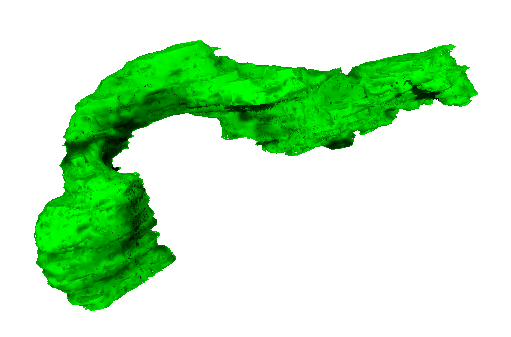
\includegraphics[scale=0.4]{Genel-Bilgiler/Figures/68gt3D.png} & 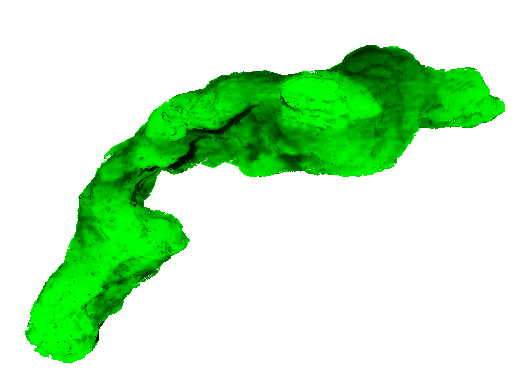
\includegraphics[scale=0.4]{Genel-Bilgiler/Figures/70gt3D.png} & 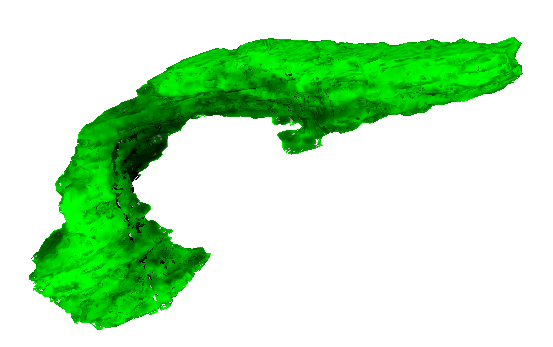
\includegraphics[scale=0.4]{Genel-Bilgiler/Figures/74gt3D.png} \\
				(d) &  (e)  & (f) 
			\end{tabular}
		}
	\end{center}
\end{figure}


Otomatik pankreas ve pankreas tümörü segmentasyonu pankreas hastalıklarına sahip kişilerin sağkalım oranını artırmak ve tanı, tedavi ve cerrahide tıp doktorlarına yardımcı olmak için kullanılmaktadır \cite{peery2019burden}. Literatür çalışmaları karaciğer, böbrek ve kalp gibi diğer abdominal organların segmentasyon başarılarının yüksek olduğunu ve tatmin edici performansların sağladığını göstermektedir \cite{peng2020method,wittenstein2019automatic,ahn2019comparative}. Oysaki Şekil \ref{fig:pancreas_types}'de görüldüğü gibi pankreasın ve pankreas tümörünün değişken büyüklükleri, şekilleri ve konumları nedeniyle, pankreas ve pankreas tümörü segmentasyonu ile ilgili çalışmalar belirli bir başarı yüzdesine kadar ulaşabilmektedirler \cite{zhao2019fully}. Tez çalışmamızın amacı literatürdeki çalışmalara göre BT görüntülemede daha yüksek doğrululuğa sahip otomatik pankreas ve pankreas tümörü segmentasyonu sağlamaktır. Bunun için bu çalışmada başarısı diğer alanlarda ispatlanmış Konvolüsyonel Sinir Ağı (Convolutional Neural Network - CNN) temelli yaklaşımlar geliştirilmektedir. Tez kapsamında gerçekleştirilen pankreas ve pankreas tümörü segmentasyonu çalışmalarının şematik temsili Şekil \ref{fig:tez_kapsami}'de gösterilmektedir. Şekil \ref{fig:tez_kapsami}'de görüldüğü gibi tez çalışması Pankreas Segmentasyonu, Pankreas ve Pankreas Tümörü Segmentasyonu olmak üzere iki ana kısımdan oluşmaktadır. 

\captionsetup[figure]{margin={0.5cm,0cm}}
\begin{figure}[h!]
	\begin{center}
		\vspace{0.4cm}
		\captionbox{Tez kapsamında gerçekleştirilen çalışmaların şematik temsili; (1) Pankreas Segmentasyonu, (2) Pankreas ve Pankreas Tümörü Segmentasyonu.
			\label{fig:tez_kapsami}}
		{
			\vspace{0.4cm}
			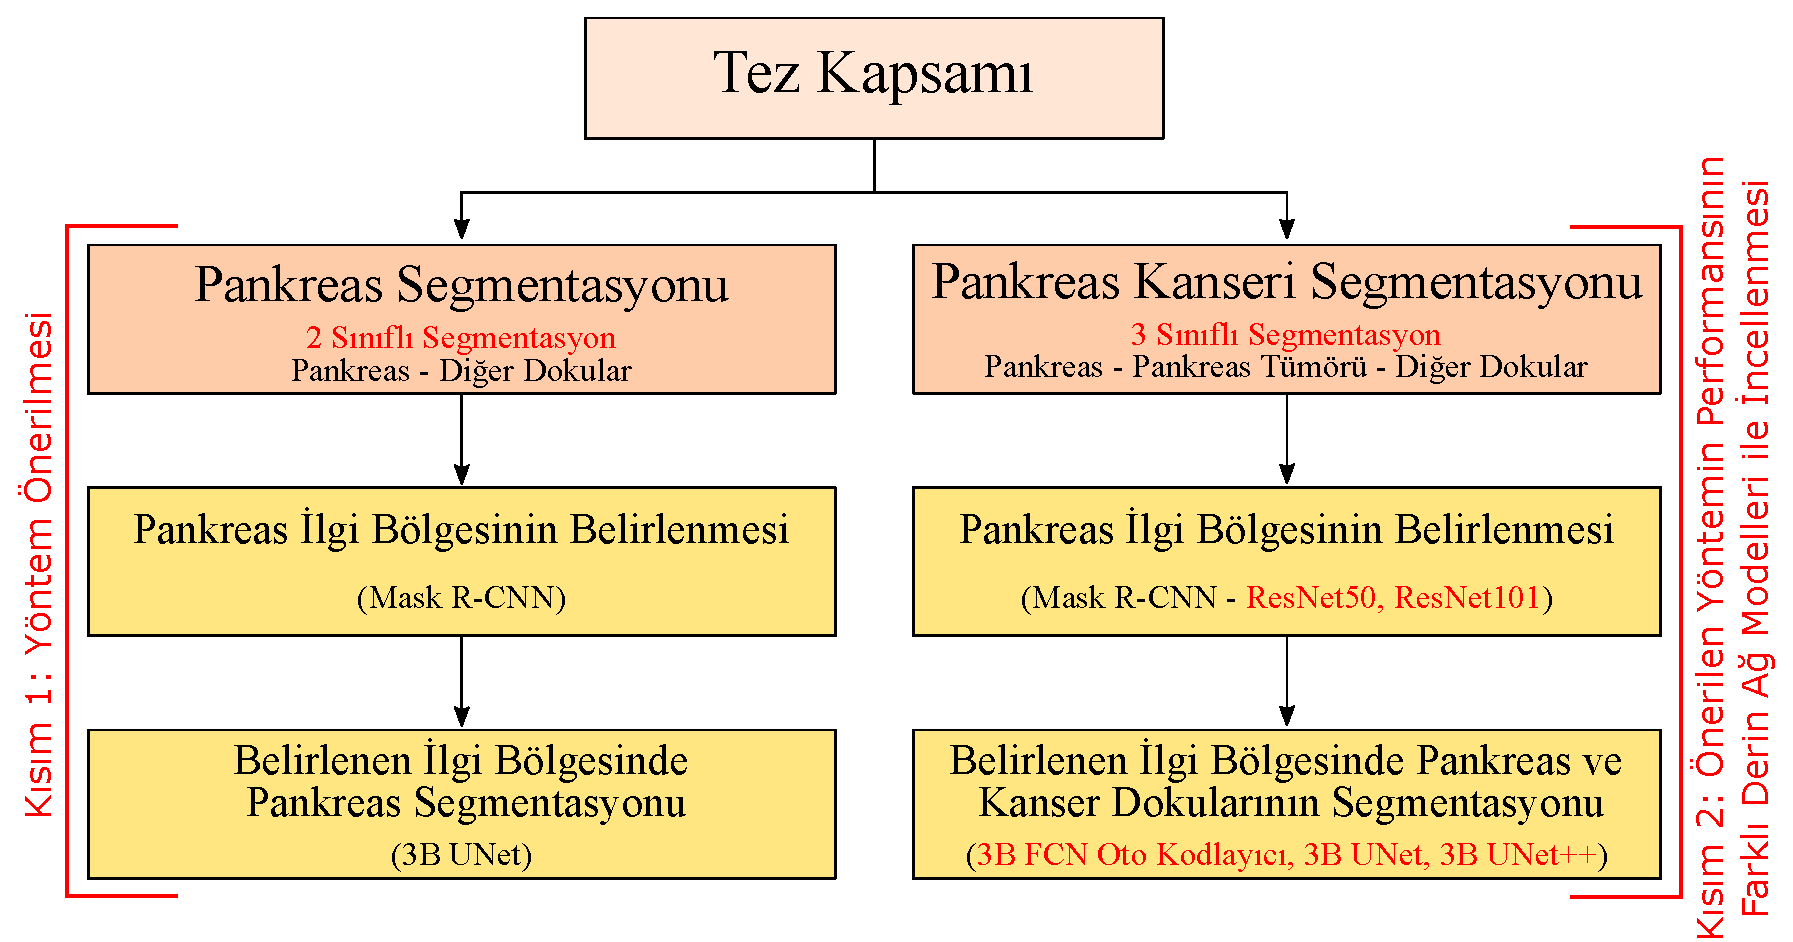
\includegraphics[scale=0.5]{Genel-Bilgiler/Figures/tezin_kapsami.pdf}
		}
	\end{center}
\end{figure}

Çalışmamızda gerçekleştirilen Pankreas Segmentasyonu kısmı Şekil \ref{fig:tez_kapsami}'de görüldüğü gibi iki ana aşamadan oluşmaktadır \cite{dogan2021two}; (i) Pankreas İlgi Bölgesinin Belirlenmesi ve (ii) Pankreas Segmentasyonu. İlk aşamada (Pankreas İlgi Bölgesinin Belirlenmesi) kaba olarak pankreas pozisyonunu tespit etmek için Maskelenmiş Bölge Esaslı Konvolüsyonel Sinir Ağı (Masked Region Proposal Convolutional Neural Network - Mask R-CNN) modeli kullanılmaktadır. Bu model tüm 2B BT dilimlerini girdi olarak almaktadır. Çıktı olarak segmente edilmiş ve maskelenmiş pankreasın aday bölgelerinin oluşturduğu 2B alt BT dilimlerini üretmektedir. İkinci aşamada (Pankreas Segmentasyonu) pankreas bölgesini daha detaylı çıkarabilmek için 3B U-Net modeli kullanılmaktadır. Bu modelde önceki aşamada üretilen 2B alt BT dilimleri girdi olarak alınmaktadır. Çıktı olarak segmente edilmiş pankreas bölgesi üretilmektedir. Pankreas segmentasyonu için önerilen yaklaşımın başarısı NIH veri setinde \cite{roth2015deep} değerlendirilmektedir. Önerilen yaklaşımın etkinliği ise performans değerlendirme metrikleri kullanılarak literatürde yüksek performans gösteren çalışmalarla karşılaştırılmaktadır. Performans değerlendirmelerinde önerilen yaklaşımın mevcut diğer yaklaşımlardan daha tatmin edici sonuçlar elde ettiği görülmektedir. 

Şekil \ref{fig:tez_kapsami}'de görüldüğü gibi tez çalışmamızın ikinci kısmı olan Pankreas ve Pankreas Tümör Segmentasyonudur. Çalışmanın Pankreas ve Pankreas Tümör Segmentasyonu kısmı da Pankreas İlgi Bölgesinin Belirlenmesi ve Pankreas ve Pankreas Tümör Segmentasyonu olmak üzere iki ana aşamadan oluşmaktadır. İlk aşamada (Pankreas İlgi Bölgesinin Belirlenmesi) kaba olarak pankreas pozisyonunu tespit etmek için Maskelenmiş Bölge Esaslı Konvolüsyonel Sinir Ağı (Masked Region Proposal Convolutional Neural Network - Mask R-CNN) modeli kullanılmaktadır. Bu model tüm 2B BT dilimlerini girdi olarak almaktadır. Çıktı olarak segmente edilmiş ve maskelenmiş pankreasın aday bölgelerinin oluşturduğu 2B alt BT dilimlerini üretmektedir. Bu modelde ResNet-50 ve Resnet-101 yapıları kullanılarak performans değerlendirmesi gerçekleştirilmektedir. İkinci aşamada (Pankreas ve Pankreas Tümör Segmentasyonu) pankreas ve pankreas tümörü bölgelerini daha detaylı çıkarabilmek için Standart Oto Kodlayıcı, 3B U-Net ve 3B U-Net++ modelleri kullanılmaktadır. Bu modellerde önceki aşamada üretilen 2B alt BT dilimleri girdi olarak alınmaktadır. Çıktı olarak segmente edilmiş pankreas ve pankreas tümör bölgeleri üretilmektedir. Pankreas ve pankreas tümör segmentasyonu için önerilen yaklaşımların başarısı Dekatlon (Medical Segmentation Decathlon - MSD) veri setinde \cite{simpson2019large} değerlendirilmektedir. Önerilen yaklaşımların etkinlikleri görmek için, çalışmamız performans değerlendirme metrikleri kullanılarak literatürde yüksek performans gösteren çalışmalarla karşılaştırılmaktadır. Performans değerlendirme metrikleri sonuçlarına göre önerilen yaklaşım mevcut diğer yaklaşımlardan daha tatmin edici segmentasyon sonuçları vermektedir. 

\subsection{Tezin Katkıları}
Tez çalışmamızın ilk kısmı olan Pankreas Segmentasyonu için önerilen yaklaşımın temel katkıları şu şekilde özetlenebilmektedir:

\begin{enumerate}
	\item Literatür çalışmaları farklı anatomik yapılara (boyut, şekil ve pozisyon) sahip pankreas gibi organların otomatik segmentasyonunun hala zorlu bir alan olduğunu göstermektedir. Bu zorluğu ortadan kaldırmak amacıyla önerilen yaklaşım bu görevi literatürdeki çalışmaların aksine, Pankreas İlgi Bölgesinin Belirlenmesi ve Pankreas Segmentasyonu olmak üzere iki ana aşamada formüle etmektedir.
	\item Daha doğru segmentasyon sonuçları üretmek, hesaplama karmaşıklığını ve maliyetini azaltmak için ilk aşamada (Pankreas İlgi Bölgesinin Belirlenmesi) obje tanıma tabanlı, gerçek zamanlı segmentasyon ve konumlandırma yapabilen Mask R-CNN modeli kullanılmaktadır.
	\item Önerilen yaklaşımın ikinci aşaması (Pankreas Segmentasyonu), önceki aşamada üretilen 2B alt BT dilimleri girdi olarak almaktadır. Bu nedenle, pankreas segmentasyonu için işlenen bölgelerin boyutu küçültülmektedir.
	\item Daha güçlü Grafik İşlemci Ünitesi (Graphics Processing Unit - GPU) kullanan literatür çalışmalarının aksine, daha düşük kapasiteli GPU kullanan tezdeki yaklaşım iki aşamadan oluşarak hem işlem belleğini azaltmakta hem de daha başarılı sonuçlar elde etmektedir.
	\item İki aşamalı yaklaşım otomatik pankreas segmentasyonu için tasarlanmış olsa da, pankreas organında görüldüğü gibi farklı yapılara sahip diğer organları segmente etmek için kolayca uyarlanabilmektedir.
	\item Önerilen yöntem pankreasın otomatik segmentasyonu için gerçek zamanlı ve tatmin edici performans sağlamaktadır.
\end{enumerate}

Tez çalışmamızın ikinci kısmı olan Pankreas ve Pankreas Tümör Segmentasyonu için önerilen yaklaşımın temel katkıları şu şekilde özetlenebilmektedir:

\begin{enumerate}
	\item Önerilen tez çalışması öncelikle Pankreas İlgi Bölgesinin Belirlenmesi aşamasında kaba pankreas bölgesini çıkarmaktadır. Daha sonra ikinci aşamada (Pankreas ve Pankreas Tümör Segmentasyonu) ilk aşamada kaba olarak bulunan pankreas bölgesinden pankreas tümör bölgesi segmente edilmektedir. Gerçekleştirilen literatür araştırmasına göre otomatik pankreas ve pankreas tümörü segmentasyonu için işlenen bölgeyi azaltarak başarıyı artıran ilk çalışmalardan biridir. 
	
	\item Otomatik pankreas tümör segmentasyonu literatürde hala zor bir alan olmasına rağmen, bu çalışmada iki aşamalı yöntem uygulanarak daha yüksek doğrulukta sonuçlar elde edilmektedir. 
	
	\item Literatür çalışmaları genellikle 2B BT görüntülerinin tüm bölgesi üzerinde otomatik pankreas tümörü segmentasyonu gerçekleştirmektedirler. Pankreas tümörlerinin farklı lokasyonları, farklı ve küçük yapıları nedeniyle tatmin edici performans sağlayamamaktadırlar. Otomatik pankreas tümörü segmentasyonu için tüm 2B BT görüntülerini işlemek yerine, önerilen yöntemimiz ilk aşamada (Pankreas İlgi Bölgesinin Belirlenmesi) kaba pankreas bölgesini tespit ederek bölgenin boyutunu küçültmektedir. 
	
	\item 2B BT görüntülerinin tüm bölgesini giriş olarak alan literatür çalışmalarından farklı olarak, bu çalışma otomatik pankreas tümörü segmentasyonu için ilk aşamada üretilen 2B alt BT görüntülerini giriş olarak almaktadır. Bu nedenle, bu çalışma daha yüksek doğruluklu pankreas tümörü segmentasyon sonuçları üretmekte, hesaplama maliyetini ve karmaşıklığını azaltmaktadır. 
	
	\item Tez çalışmasında otomatik pankreas tümörü segmentasyonu için ilk aşamada (Pankreas İlgi Bölgesinin Belirlenmesi) üretilen 2B alt BT görüntülerinin işlenmesi nedeniyle, GPU kapasitesi daha düşük olan çalışmamız, daha güçlü GPU kapasiteli diğer literatür çalışmalarına göre daha yüksek doğrulukta sonuçlar üretebilmektedir. 
	
\end{enumerate}
